%&latex
% Copyright 2011 Zoresvit (c) <zoresvit@gmail.com>

\documentclass[10pt, ucs, handout]{beamer}
\usefonttheme[onlymath]{serif}
\usetheme{zslides}
\usepackage{xcolor}
\usepackage{tikz}

\graphicspath{{images/}}
\setbeamercolor{alerted text}{fg=red!50!black}

\usepackage{pgfpages}
\pgfpagesuselayout{2 on 1}[a4paper,border shrink=5mm]
\mode<handout>{\setbeamercolor{background canvas}{bg=black!5}}

\addtobeamertemplate{title page}{%
\vspace*{2ex}\large\centering Харківський національний університет радіоелектроніки\\
}{}

\newcommand{\worktitle}{Аналіз криптографічних властивостей симетричних шифрів \\[2ex]}
\newcommand{\workauthors}{Руслан Кіянчук}


\title[Криптографічні властивості симетричних шифрів]{\worktitle}
\author[\workauthors]{
    \texorpdfstring{Руслан Кіянчук\\[2ex]
    \scriptsize\url{ruslan.kiyanchuk@gmail.com}}{\workauthors} \\[4ex]%
    \begin{flushleft}
    \hspace*{10em}
    \normalsize Науковий керівник: \hspace*{10ex} Халімов Г. З. \\[0.8ex]
    \hspace*{6.9em}
    \normalsize Консультант: \hspace*{15.8ex} Олійников Р. В.
\end{flushleft} \\[-8ex]
}

\subtitle{Бакалаврська робота}
\institute[ХНУРЕ]{}
\date[Харків 2012]{\normalsize Харків 2012}

\hypersetup{
pdftitle = {\worktitle},
pdfauthor = {\workauthors}, 
pdfkeywords = {}
}


\begin{document}
\selectlanguage{ukrainian}
\maketitle

\section{Актуальність}
\begin{frame}{Актуальність}{Нагальні проблеми}
    \small
    \begin{block}{}
        \begin{itemize}
            \item Сучасні криптоалгоритми базуються на складній математиці.
            \item Реальні системи безпеки часто є вразливими із-за некоректного
                використання та помилок реалізації.
        \end{itemize}
    \end{block}
    \alert{стандарт GSM:}
    \begin{description}
        \item[A5/1] можливо зламати за секунди
            (використовуючи~rainbow~таблиці).
    \end{description}
    \alert{Супутникові телефони:}
    \begin{description}
        \item[GMR-1] базується на A5/2 (виведений з експлуатації з 2007~р.);
        \item[GMR-2] неопублікований алгоритм (атака потребує $65$~б гами).
    \end{description}
    \alert{Безпровідний інтернет:}
    \begin{description}
        \item [WEP] необхідно $80000$ пакетів для проведення криптоаналізу;
        \item[E0] атака вимагає $2^{38}$ операцій та $2^{23.8}$~фрагментів
            даних.
    \end{description}
    \begin{block}{}
        Необхідно проводити детальний аналіз та відкриту експертизу шифрів
        перед застосуванням у реальних системах безпеки.
    \end{block}
\end{frame}

\begin{frame}[shrink=1.2]{Актуальність}{Напрями розвитку криптографії}
    \footnotesize
    \onslide<1->{
    \begin{block}{Мало-ресурсна (lightweight) криптографія}
        \begin{itemize}
            \item портативні пристрої мають забезпечувати безпеку даних;
            \item обчислювальні ресурси є обмеженими;
            \item необхідні шифри, що мають ефективну апаратну реалізацію.
        \end{itemize}    
    \end{block}
    }
    \onslide<2->{
    \begin{block}{Стандарти мобільного зв'язку}
        \begin{itemize}
            \item потрібні нові шифри для для захисту даних наступного
                покоління зв'язку LTE;
            \item ZUC --- китайський шифр, розроблений у 2011~р.;
            \item шифр проходить період відкритої експертизи.
        \end{itemize}
    \end{block}
    }
    \onslide<3->{
    \begin{block}{Актуальність ГОСТ~28147}
        \begin{itemize}
            \item прийнятий у 1989~р. стандарт шифрування ГОСТ широко
                застосовується в Україні та країнах СНД;
            \item запропонований для стандартизації в ISO у 2010 р;
            \item перспективний для використання у мало-ресурсній криптографії;
            \item відсутня оцінка стійкості до алгебраїчного криптоаналізу.
        \end{itemize}
    \end{block}
    }
\end{frame}

\section{Криптографічні властивості шифра ZUC}
\begin{frame}{Поточний шифр ZUC}{Перспективний для використання в LTE}
    \begin{minipage}{0.4 \textwidth}
        \begin{itemize}
            \item 16 елементів над {\small $GF(p) = GF(2^{31}-1)$};
            \item період $p^{16} -1 \approx 2^{496}$;
            \item $X_0 = s_{15_H} || s_{14_L}$,  \\ 
                $X_1 = s_{11_L} || s_{14_H}$, \\ 
                $X_2 = s_{7_L} || s_{5_H}$, \\ 
                $X_3 = s_{2_L} || s_{0_H}$;
            \item $R_1$, $R_2$ -- регістри;
            \item $L_1$, $L_2$ лінійні перетворення --
                поліноми над $GF(2)[x]/(x^{32}+1)$;
            \item $S \rightarrow (S_0, S_1, S_0, S_1)$.
        \end{itemize}
        \begin{block}{}
            Виявлено недолік лінійного перетворення шифра.
        \end{block}
    \end{minipage}%
        \hspace*{1.6ex}%
    \begin{minipage}{0.6 \textwidth}
        % Graphic for TeX using PGF
% Title: /home/zoresvit/Documents/research/diploma/graphics/zuc.dia
% Creator: Dia v0.97.1
% CreationDate: Fri Nov 11 01:43:40 2011
% For: zoresvit
% \usepackage{tikz}
% The following commands are not supported in PSTricks at present
% We define them conditionally, so when they are implemented,
% this pgf file will use them.
\ifx\du\undefined
  \newlength{\du}
\fi
\setlength{\du}{10\unitlength}

\begin{tikzpicture}[scale=0.55,every node/.style={scale=0.6}]

\pgftransformxscale{1.000000}
\pgftransformyscale{-1.000000}
\definecolor{dialinecolor}{rgb}{0.000000, 0.000000, 0.000000}
\pgfsetstrokecolor{dialinecolor}
\definecolor{dialinecolor}{rgb}{1.000000, 1.000000, 1.000000}
\pgfsetfillcolor{dialinecolor}
\pgfsetlinewidth{0.100000\du}
\pgfsetdash{{\pgflinewidth}{0.200000\du}}{0cm}
\pgfsetdash{{\pgflinewidth}{0.200000\du}}{0cm}
\pgfsetmiterjoin
\definecolor{dialinecolor}{rgb}{0.000000, 0.000000, 0.000000}
\pgfsetstrokecolor{dialinecolor}
\draw (7.000000\du,-3.000000\du)--(7.000000\du,7.000000\du)--(43.500000\du,7.000000\du)--(43.500000\du,-3.000000\du)--cycle;
% setfont left to latex
\definecolor{dialinecolor}{rgb}{0.000000, 0.000000, 0.000000}
\pgfsetstrokecolor{dialinecolor}
\node at (25.250000\du,2.195000\du){};
\pgfsetlinewidth{0.100000\du}
\pgfsetdash{{\pgflinewidth}{0.200000\du}}{0cm}
\pgfsetdash{{\pgflinewidth}{0.200000\du}}{0cm}
\pgfsetmiterjoin
\definecolor{dialinecolor}{rgb}{0.000000, 0.000000, 0.000000}
\pgfsetstrokecolor{dialinecolor}
\draw (7.000000\du,8.000000\du)--(7.000000\du,12.000000\du)--(43.500000\du,12.000000\du)--(43.500000\du,8.000000\du)--cycle;
% setfont left to latex
\definecolor{dialinecolor}{rgb}{0.000000, 0.000000, 0.000000}
\pgfsetstrokecolor{dialinecolor}
\node at (25.250000\du,10.195000\du){};
\pgfsetlinewidth{0.100000\du}
\pgfsetdash{{\pgflinewidth}{0.200000\du}}{0cm}
\pgfsetdash{{\pgflinewidth}{0.200000\du}}{0cm}
\pgfsetmiterjoin
\definecolor{dialinecolor}{rgb}{0.000000, 0.000000, 0.000000}
\pgfsetstrokecolor{dialinecolor}
\draw (7.100000\du,13.000000\du)--(7.100000\du,34.000000\du)--(32.100000\du,34.000000\du)--(32.100000\du,13.000000\du)--cycle;
% setfont left to latex
\definecolor{dialinecolor}{rgb}{0.000000, 0.000000, 0.000000}
\pgfsetstrokecolor{dialinecolor}
\node at (19.600000\du,23.695000\du){};
% setfont left to latex
\definecolor{dialinecolor}{rgb}{0.000000, 0.000000, 0.000000}
\pgfsetstrokecolor{dialinecolor}
\node[anchor=west] at (25.500000\du,1.500000\du){LFSR};
% setfont left to latex
\definecolor{dialinecolor}{rgb}{0.000000, 0.000000, 0.000000}
\pgfsetstrokecolor{dialinecolor}
\node[anchor=west] at (24.500000\du,9.000000\du){BR};
\definecolor{dialinecolor}{rgb}{1.000000, 1.000000, 1.000000}
\pgfsetfillcolor{dialinecolor}
\fill (40.000000\du,4.000000\du)--(40.000000\du,6.000000\du)--(42.000000\du,6.000000\du)--(42.000000\du,4.000000\du)--cycle;
\pgfsetlinewidth{0.100000\du}
\pgfsetdash{}{0pt}
\pgfsetdash{}{0pt}
\pgfsetmiterjoin
\definecolor{dialinecolor}{rgb}{0.000000, 0.000000, 0.000000}
\pgfsetstrokecolor{dialinecolor}
\draw (40.000000\du,4.000000\du)--(40.000000\du,6.000000\du)--(42.000000\du,6.000000\du)--(42.000000\du,4.000000\du)--cycle;
% setfont left to latex
\definecolor{dialinecolor}{rgb}{0.000000, 0.000000, 0.000000}
\pgfsetstrokecolor{dialinecolor}
\node at (41.000000\du,5.195000\du){$s_{0}$};
\definecolor{dialinecolor}{rgb}{1.000000, 1.000000, 1.000000}
\pgfsetfillcolor{dialinecolor}
\fill (38.000000\du,4.000000\du)--(38.000000\du,6.000000\du)--(40.000000\du,6.000000\du)--(40.000000\du,4.000000\du)--cycle;
\pgfsetlinewidth{0.100000\du}
\pgfsetdash{}{0pt}
\pgfsetdash{}{0pt}
\pgfsetmiterjoin
\definecolor{dialinecolor}{rgb}{0.000000, 0.000000, 0.000000}
\pgfsetstrokecolor{dialinecolor}
\draw (38.000000\du,4.000000\du)--(38.000000\du,6.000000\du)--(40.000000\du,6.000000\du)--(40.000000\du,4.000000\du)--cycle;
% setfont left to latex
\definecolor{dialinecolor}{rgb}{0.000000, 0.000000, 0.000000}
\pgfsetstrokecolor{dialinecolor}
\node at (39.000000\du,5.195000\du){$s_{1}$};
\definecolor{dialinecolor}{rgb}{1.000000, 1.000000, 1.000000}
\pgfsetfillcolor{dialinecolor}
\fill (36.000000\du,4.000000\du)--(36.000000\du,6.000000\du)--(38.000000\du,6.000000\du)--(38.000000\du,4.000000\du)--cycle;
\pgfsetlinewidth{0.100000\du}
\pgfsetdash{}{0pt}
\pgfsetdash{}{0pt}
\pgfsetmiterjoin
\definecolor{dialinecolor}{rgb}{0.000000, 0.000000, 0.000000}
\pgfsetstrokecolor{dialinecolor}
\draw (36.000000\du,4.000000\du)--(36.000000\du,6.000000\du)--(38.000000\du,6.000000\du)--(38.000000\du,4.000000\du)--cycle;
% setfont left to latex
\definecolor{dialinecolor}{rgb}{0.000000, 0.000000, 0.000000}
\pgfsetstrokecolor{dialinecolor}
\node at (37.000000\du,5.195000\du){$s_{2}$};
\definecolor{dialinecolor}{rgb}{1.000000, 1.000000, 1.000000}
\pgfsetfillcolor{dialinecolor}
\fill (34.000000\du,4.000000\du)--(34.000000\du,6.000000\du)--(36.000000\du,6.000000\du)--(36.000000\du,4.000000\du)--cycle;
\pgfsetlinewidth{0.100000\du}
\pgfsetdash{}{0pt}
\pgfsetdash{}{0pt}
\pgfsetmiterjoin
\definecolor{dialinecolor}{rgb}{0.000000, 0.000000, 0.000000}
\pgfsetstrokecolor{dialinecolor}
\draw (34.000000\du,4.000000\du)--(34.000000\du,6.000000\du)--(36.000000\du,6.000000\du)--(36.000000\du,4.000000\du)--cycle;
% setfont left to latex
\definecolor{dialinecolor}{rgb}{0.000000, 0.000000, 0.000000}
\pgfsetstrokecolor{dialinecolor}
\node at (35.000000\du,5.195000\du){$s_{3}$};
\definecolor{dialinecolor}{rgb}{1.000000, 1.000000, 1.000000}
\pgfsetfillcolor{dialinecolor}
\fill (32.000000\du,4.000000\du)--(32.000000\du,6.000000\du)--(34.000000\du,6.000000\du)--(34.000000\du,4.000000\du)--cycle;
\pgfsetlinewidth{0.100000\du}
\pgfsetdash{}{0pt}
\pgfsetdash{}{0pt}
\pgfsetmiterjoin
\definecolor{dialinecolor}{rgb}{0.000000, 0.000000, 0.000000}
\pgfsetstrokecolor{dialinecolor}
\draw (32.000000\du,4.000000\du)--(32.000000\du,6.000000\du)--(34.000000\du,6.000000\du)--(34.000000\du,4.000000\du)--cycle;
% setfont left to latex
\definecolor{dialinecolor}{rgb}{0.000000, 0.000000, 0.000000}
\pgfsetstrokecolor{dialinecolor}
\node at (33.000000\du,5.195000\du){$s_{4}$};
\definecolor{dialinecolor}{rgb}{1.000000, 1.000000, 1.000000}
\pgfsetfillcolor{dialinecolor}
\fill (30.000000\du,4.000000\du)--(30.000000\du,6.000000\du)--(32.000000\du,6.000000\du)--(32.000000\du,4.000000\du)--cycle;
\pgfsetlinewidth{0.100000\du}
\pgfsetdash{}{0pt}
\pgfsetdash{}{0pt}
\pgfsetmiterjoin
\definecolor{dialinecolor}{rgb}{0.000000, 0.000000, 0.000000}
\pgfsetstrokecolor{dialinecolor}
\draw (30.000000\du,4.000000\du)--(30.000000\du,6.000000\du)--(32.000000\du,6.000000\du)--(32.000000\du,4.000000\du)--cycle;
% setfont left to latex
\definecolor{dialinecolor}{rgb}{0.000000, 0.000000, 0.000000}
\pgfsetstrokecolor{dialinecolor}
\node at (31.000000\du,5.195000\du){$s_{5}$};
\definecolor{dialinecolor}{rgb}{1.000000, 1.000000, 1.000000}
\pgfsetfillcolor{dialinecolor}
\fill (28.000000\du,4.000000\du)--(28.000000\du,6.000000\du)--(30.000000\du,6.000000\du)--(30.000000\du,4.000000\du)--cycle;
\pgfsetlinewidth{0.100000\du}
\pgfsetdash{}{0pt}
\pgfsetdash{}{0pt}
\pgfsetmiterjoin
\definecolor{dialinecolor}{rgb}{0.000000, 0.000000, 0.000000}
\pgfsetstrokecolor{dialinecolor}
\draw (28.000000\du,4.000000\du)--(28.000000\du,6.000000\du)--(30.000000\du,6.000000\du)--(30.000000\du,4.000000\du)--cycle;
% setfont left to latex
\definecolor{dialinecolor}{rgb}{0.000000, 0.000000, 0.000000}
\pgfsetstrokecolor{dialinecolor}
\node at (29.000000\du,5.195000\du){$s_{6}$};
\definecolor{dialinecolor}{rgb}{1.000000, 1.000000, 1.000000}
\pgfsetfillcolor{dialinecolor}
\fill (26.000000\du,4.000000\du)--(26.000000\du,6.000000\du)--(28.000000\du,6.000000\du)--(28.000000\du,4.000000\du)--cycle;
\pgfsetlinewidth{0.100000\du}
\pgfsetdash{}{0pt}
\pgfsetdash{}{0pt}
\pgfsetmiterjoin
\definecolor{dialinecolor}{rgb}{0.000000, 0.000000, 0.000000}
\pgfsetstrokecolor{dialinecolor}
\draw (26.000000\du,4.000000\du)--(26.000000\du,6.000000\du)--(28.000000\du,6.000000\du)--(28.000000\du,4.000000\du)--cycle;
% setfont left to latex
\definecolor{dialinecolor}{rgb}{0.000000, 0.000000, 0.000000}
\pgfsetstrokecolor{dialinecolor}
\node at (27.000000\du,5.195000\du){$s_{7}$};
\definecolor{dialinecolor}{rgb}{1.000000, 1.000000, 1.000000}
\pgfsetfillcolor{dialinecolor}
\fill (24.000000\du,4.000000\du)--(24.000000\du,6.000000\du)--(26.000000\du,6.000000\du)--(26.000000\du,4.000000\du)--cycle;
\pgfsetlinewidth{0.100000\du}
\pgfsetdash{}{0pt}
\pgfsetdash{}{0pt}
\pgfsetmiterjoin
\definecolor{dialinecolor}{rgb}{0.000000, 0.000000, 0.000000}
\pgfsetstrokecolor{dialinecolor}
\draw (24.000000\du,4.000000\du)--(24.000000\du,6.000000\du)--(26.000000\du,6.000000\du)--(26.000000\du,4.000000\du)--cycle;
% setfont left to latex
\definecolor{dialinecolor}{rgb}{0.000000, 0.000000, 0.000000}
\pgfsetstrokecolor{dialinecolor}
\node at (25.000000\du,5.195000\du){$s_{8}$};
\definecolor{dialinecolor}{rgb}{1.000000, 1.000000, 1.000000}
\pgfsetfillcolor{dialinecolor}
\fill (22.000000\du,4.000000\du)--(22.000000\du,6.000000\du)--(24.000000\du,6.000000\du)--(24.000000\du,4.000000\du)--cycle;
\pgfsetlinewidth{0.100000\du}
\pgfsetdash{}{0pt}
\pgfsetdash{}{0pt}
\pgfsetmiterjoin
\definecolor{dialinecolor}{rgb}{0.000000, 0.000000, 0.000000}
\pgfsetstrokecolor{dialinecolor}
\draw (22.000000\du,4.000000\du)--(22.000000\du,6.000000\du)--(24.000000\du,6.000000\du)--(24.000000\du,4.000000\du)--cycle;
% setfont left to latex
\definecolor{dialinecolor}{rgb}{0.000000, 0.000000, 0.000000}
\pgfsetstrokecolor{dialinecolor}
\node at (23.000000\du,5.195000\du){$s_{9}$};
\definecolor{dialinecolor}{rgb}{1.000000, 1.000000, 1.000000}
\pgfsetfillcolor{dialinecolor}
\fill (19.800000\du,4.000000\du)--(19.800000\du,6.000000\du)--(22.050000\du,6.000000\du)--(22.050000\du,4.000000\du)--cycle;
\pgfsetlinewidth{0.100000\du}
\pgfsetdash{}{0pt}
\pgfsetdash{}{0pt}
\pgfsetmiterjoin
\definecolor{dialinecolor}{rgb}{0.000000, 0.000000, 0.000000}
\pgfsetstrokecolor{dialinecolor}
\draw (19.800000\du,4.000000\du)--(19.800000\du,6.000000\du)--(22.050000\du,6.000000\du)--(22.050000\du,4.000000\du)--cycle;
% setfont left to latex
\definecolor{dialinecolor}{rgb}{0.000000, 0.000000, 0.000000}
\pgfsetstrokecolor{dialinecolor}
\node at (20.925000\du,5.195000\du){$s_{10}$};
\definecolor{dialinecolor}{rgb}{1.000000, 1.000000, 1.000000}
\pgfsetfillcolor{dialinecolor}
\fill (17.800000\du,4.000000\du)--(17.800000\du,6.000000\du)--(20.050000\du,6.000000\du)--(20.050000\du,4.000000\du)--cycle;
\pgfsetlinewidth{0.100000\du}
\pgfsetdash{}{0pt}
\pgfsetdash{}{0pt}
\pgfsetmiterjoin
\definecolor{dialinecolor}{rgb}{0.000000, 0.000000, 0.000000}
\pgfsetstrokecolor{dialinecolor}
\draw (17.800000\du,4.000000\du)--(17.800000\du,6.000000\du)--(20.050000\du,6.000000\du)--(20.050000\du,4.000000\du)--cycle;
% setfont left to latex
\definecolor{dialinecolor}{rgb}{0.000000, 0.000000, 0.000000}
\pgfsetstrokecolor{dialinecolor}
\node at (18.925000\du,5.195000\du){$s_{11}$};
\definecolor{dialinecolor}{rgb}{1.000000, 1.000000, 1.000000}
\pgfsetfillcolor{dialinecolor}
\fill (15.600000\du,4.000000\du)--(15.600000\du,6.000000\du)--(17.850000\du,6.000000\du)--(17.850000\du,4.000000\du)--cycle;
\pgfsetlinewidth{0.100000\du}
\pgfsetdash{}{0pt}
\pgfsetdash{}{0pt}
\pgfsetmiterjoin
\definecolor{dialinecolor}{rgb}{0.000000, 0.000000, 0.000000}
\pgfsetstrokecolor{dialinecolor}
\draw (15.600000\du,4.000000\du)--(15.600000\du,6.000000\du)--(17.850000\du,6.000000\du)--(17.850000\du,4.000000\du)--cycle;
% setfont left to latex
\definecolor{dialinecolor}{rgb}{0.000000, 0.000000, 0.000000}
\pgfsetstrokecolor{dialinecolor}
\node at (16.725000\du,5.195000\du){$s_{12}$};
\definecolor{dialinecolor}{rgb}{1.000000, 1.000000, 1.000000}
\pgfsetfillcolor{dialinecolor}
\fill (13.475000\du,4.000000\du)--(13.475000\du,6.000000\du)--(15.725000\du,6.000000\du)--(15.725000\du,4.000000\du)--cycle;
\pgfsetlinewidth{0.100000\du}
\pgfsetdash{}{0pt}
\pgfsetdash{}{0pt}
\pgfsetmiterjoin
\definecolor{dialinecolor}{rgb}{0.000000, 0.000000, 0.000000}
\pgfsetstrokecolor{dialinecolor}
\draw (13.475000\du,4.000000\du)--(13.475000\du,6.000000\du)--(15.725000\du,6.000000\du)--(15.725000\du,4.000000\du)--cycle;
% setfont left to latex
\definecolor{dialinecolor}{rgb}{0.000000, 0.000000, 0.000000}
\pgfsetstrokecolor{dialinecolor}
\node at (14.600000\du,5.195000\du){$s_{13}$};
\definecolor{dialinecolor}{rgb}{1.000000, 1.000000, 1.000000}
\pgfsetfillcolor{dialinecolor}
\fill (11.275000\du,4.000000\du)--(11.275000\du,6.000000\du)--(13.525000\du,6.000000\du)--(13.525000\du,4.000000\du)--cycle;
\pgfsetlinewidth{0.100000\du}
\pgfsetdash{}{0pt}
\pgfsetdash{}{0pt}
\pgfsetmiterjoin
\definecolor{dialinecolor}{rgb}{0.000000, 0.000000, 0.000000}
\pgfsetstrokecolor{dialinecolor}
\draw (11.275000\du,4.000000\du)--(11.275000\du,6.000000\du)--(13.525000\du,6.000000\du)--(13.525000\du,4.000000\du)--cycle;
% setfont left to latex
\definecolor{dialinecolor}{rgb}{0.000000, 0.000000, 0.000000}
\pgfsetstrokecolor{dialinecolor}
\node at (12.400000\du,5.195000\du){$s_{14}$};
\definecolor{dialinecolor}{rgb}{1.000000, 1.000000, 1.000000}
\pgfsetfillcolor{dialinecolor}
\fill (9.000000\du,4.000000\du)--(9.000000\du,6.000000\du)--(11.250000\du,6.000000\du)--(11.250000\du,4.000000\du)--cycle;
\pgfsetlinewidth{0.100000\du}
\pgfsetdash{}{0pt}
\pgfsetdash{}{0pt}
\pgfsetmiterjoin
\definecolor{dialinecolor}{rgb}{0.000000, 0.000000, 0.000000}
\pgfsetstrokecolor{dialinecolor}
\draw (9.000000\du,4.000000\du)--(9.000000\du,6.000000\du)--(11.250000\du,6.000000\du)--(11.250000\du,4.000000\du)--cycle;
% setfont left to latex
\definecolor{dialinecolor}{rgb}{0.000000, 0.000000, 0.000000}
\pgfsetstrokecolor{dialinecolor}
\node at (10.125000\du,5.195000\du){$s_{15}$};
\definecolor{dialinecolor}{rgb}{1.000000, 1.000000, 1.000000}
\pgfsetfillcolor{dialinecolor}
\fill (9.000000\du,-2.000000\du)--(9.000000\du,0.000000\du)--(42.000000\du,0.000000\du)--(42.000000\du,-2.000000\du)--cycle;
\pgfsetlinewidth{0.100000\du}
\pgfsetdash{}{0pt}
\pgfsetdash{}{0pt}
\pgfsetmiterjoin
\definecolor{dialinecolor}{rgb}{0.000000, 0.000000, 0.000000}
\pgfsetstrokecolor{dialinecolor}
\draw (9.000000\du,-2.000000\du)--(9.000000\du,0.000000\du)--(42.000000\du,0.000000\du)--(42.000000\du,-2.000000\du)--cycle;
% setfont left to latex
\definecolor{dialinecolor}{rgb}{0.000000, 0.000000, 0.000000}
\pgfsetstrokecolor{dialinecolor}
\node at (25.500000\du,-0.805000\du){$\mod 2^{31} - 1$};
\pgfsetlinewidth{0.100000\du}
\pgfsetdash{}{0pt}
\pgfsetdash{}{0pt}
\pgfsetbuttcap
\pgfsetmiterjoin
\pgfsetlinewidth{0.100000\du}
\pgfsetbuttcap
\pgfsetmiterjoin
\pgfsetdash{}{0pt}
\definecolor{dialinecolor}{rgb}{1.000000, 1.000000, 1.000000}
\pgfsetfillcolor{dialinecolor}
\pgfpathmoveto{\pgfpoint{39.655000\du}{1.200000\du}}
\pgfpathlineto{\pgfpoint{41.475000\du}{1.200000\du}}
\pgfpathcurveto{\pgfpoint{41.726290\du}{1.200000\du}}{\pgfpoint{41.930000\du}{1.513401\du}}{\pgfpoint{41.930000\du}{1.900000\du}}
\pgfpathcurveto{\pgfpoint{41.930000\du}{2.286600\du}}{\pgfpoint{41.726290\du}{2.600000\du}}{\pgfpoint{41.475000\du}{2.600000\du}}
\pgfpathlineto{\pgfpoint{39.655000\du}{2.600000\du}}
\pgfpathcurveto{\pgfpoint{39.403710\du}{2.600000\du}}{\pgfpoint{39.200000\du}{2.286600\du}}{\pgfpoint{39.200000\du}{1.900000\du}}
\pgfpathcurveto{\pgfpoint{39.200000\du}{1.513401\du}}{\pgfpoint{39.403710\du}{1.200000\du}}{\pgfpoint{39.655000\du}{1.200000\du}}
\pgfusepath{fill}
\definecolor{dialinecolor}{rgb}{0.000000, 0.000000, 0.000000}
\pgfsetstrokecolor{dialinecolor}
\pgfpathmoveto{\pgfpoint{39.655000\du}{1.200000\du}}
\pgfpathlineto{\pgfpoint{41.475000\du}{1.200000\du}}
\pgfpathcurveto{\pgfpoint{41.726290\du}{1.200000\du}}{\pgfpoint{41.930000\du}{1.513401\du}}{\pgfpoint{41.930000\du}{1.900000\du}}
\pgfpathcurveto{\pgfpoint{41.930000\du}{2.286600\du}}{\pgfpoint{41.726290\du}{2.600000\du}}{\pgfpoint{41.475000\du}{2.600000\du}}
\pgfpathlineto{\pgfpoint{39.655000\du}{2.600000\du}}
\pgfpathcurveto{\pgfpoint{39.403710\du}{2.600000\du}}{\pgfpoint{39.200000\du}{2.286600\du}}{\pgfpoint{39.200000\du}{1.900000\du}}
\pgfpathcurveto{\pgfpoint{39.200000\du}{1.513401\du}}{\pgfpoint{39.403710\du}{1.200000\du}}{\pgfpoint{39.655000\du}{1.200000\du}}
\pgfusepath{stroke}
% setfont left to latex
\definecolor{dialinecolor}{rgb}{0.000000, 0.000000, 0.000000}
\pgfsetstrokecolor{dialinecolor}
\node at (40.565000\du,2.032292\du){$\scriptstyle 2^8 + 1$};
\pgfsetlinewidth{0.100000\du}
\pgfsetdash{}{0pt}
\pgfsetdash{}{0pt}
\pgfsetbuttcap
{
\definecolor{dialinecolor}{rgb}{0.000000, 0.000000, 0.000000}
\pgfsetfillcolor{dialinecolor}
% was here!!!
\pgfsetarrowsend{latex}
\definecolor{dialinecolor}{rgb}{0.000000, 0.000000, 0.000000}
\pgfsetstrokecolor{dialinecolor}
\draw (41.000000\du,3.949707\du)--(41.000000\du,2.600000\du);
}
\pgfsetlinewidth{0.100000\du}
\pgfsetdash{}{0pt}
\pgfsetdash{}{0pt}
\pgfsetbuttcap
{
\definecolor{dialinecolor}{rgb}{0.000000, 0.000000, 0.000000}
\pgfsetfillcolor{dialinecolor}
% was here!!!
\pgfsetarrowsend{latex}
\definecolor{dialinecolor}{rgb}{0.000000, 0.000000, 0.000000}
\pgfsetstrokecolor{dialinecolor}
\draw (41.020000\du,1.200000\du)--(41.000000\du,0.000000\du);
}
\pgfsetlinewidth{0.100000\du}
\pgfsetdash{}{0pt}
\pgfsetdash{}{0pt}
\pgfsetbuttcap
\pgfsetmiterjoin
\pgfsetlinewidth{0.100000\du}
\pgfsetbuttcap
\pgfsetmiterjoin
\pgfsetdash{}{0pt}
\definecolor{dialinecolor}{rgb}{1.000000, 1.000000, 1.000000}
\pgfsetfillcolor{dialinecolor}
\pgfpathmoveto{\pgfpoint{32.366250\du}{1.200000\du}}
\pgfpathlineto{\pgfpoint{33.831250\du}{1.200000\du}}
\pgfpathcurveto{\pgfpoint{34.033524\du}{1.200000\du}}{\pgfpoint{34.197500\du}{1.513401\du}}{\pgfpoint{34.197500\du}{1.900000\du}}
\pgfpathcurveto{\pgfpoint{34.197500\du}{2.286600\du}}{\pgfpoint{34.033524\du}{2.600000\du}}{\pgfpoint{33.831250\du}{2.600000\du}}
\pgfpathlineto{\pgfpoint{32.366250\du}{2.600000\du}}
\pgfpathcurveto{\pgfpoint{32.163976\du}{2.600000\du}}{\pgfpoint{32.000000\du}{2.286600\du}}{\pgfpoint{32.000000\du}{1.900000\du}}
\pgfpathcurveto{\pgfpoint{32.000000\du}{1.513401\du}}{\pgfpoint{32.163976\du}{1.200000\du}}{\pgfpoint{32.366250\du}{1.200000\du}}
\pgfusepath{fill}
\definecolor{dialinecolor}{rgb}{0.000000, 0.000000, 0.000000}
\pgfsetstrokecolor{dialinecolor}
\pgfpathmoveto{\pgfpoint{32.366250\du}{1.200000\du}}
\pgfpathlineto{\pgfpoint{33.831250\du}{1.200000\du}}
\pgfpathcurveto{\pgfpoint{34.033524\du}{1.200000\du}}{\pgfpoint{34.197500\du}{1.513401\du}}{\pgfpoint{34.197500\du}{1.900000\du}}
\pgfpathcurveto{\pgfpoint{34.197500\du}{2.286600\du}}{\pgfpoint{34.033524\du}{2.600000\du}}{\pgfpoint{33.831250\du}{2.600000\du}}
\pgfpathlineto{\pgfpoint{32.366250\du}{2.600000\du}}
\pgfpathcurveto{\pgfpoint{32.163976\du}{2.600000\du}}{\pgfpoint{32.000000\du}{2.286600\du}}{\pgfpoint{32.000000\du}{1.900000\du}}
\pgfpathcurveto{\pgfpoint{32.000000\du}{1.513401\du}}{\pgfpoint{32.163976\du}{1.200000\du}}{\pgfpoint{32.366250\du}{1.200000\du}}
\pgfusepath{stroke}
% setfont left to latex
\definecolor{dialinecolor}{rgb}{0.000000, 0.000000, 0.000000}
\pgfsetstrokecolor{dialinecolor}
\node at (33.098750\du,2.032292\du){$2^{20}$};
\pgfsetlinewidth{0.100000\du}
\pgfsetdash{}{0pt}
\pgfsetdash{}{0pt}
\pgfsetbuttcap
{
\definecolor{dialinecolor}{rgb}{0.000000, 0.000000, 0.000000}
\pgfsetfillcolor{dialinecolor}
% was here!!!
\pgfsetarrowsend{latex}
\definecolor{dialinecolor}{rgb}{0.000000, 0.000000, 0.000000}
\pgfsetstrokecolor{dialinecolor}
\draw (33.000000\du,4.000000\du)--(33.000000\du,2.600000\du);
}
\pgfsetlinewidth{0.100000\du}
\pgfsetdash{}{0pt}
\pgfsetdash{}{0pt}
\pgfsetbuttcap
{
\definecolor{dialinecolor}{rgb}{0.000000, 0.000000, 0.000000}
\pgfsetfillcolor{dialinecolor}
% was here!!!
\pgfsetarrowsend{latex}
\definecolor{dialinecolor}{rgb}{0.000000, 0.000000, 0.000000}
\pgfsetstrokecolor{dialinecolor}
\draw (33.000000\du,1.200000\du)--(33.000000\du,0.000000\du);
}
\pgfsetlinewidth{0.100000\du}
\pgfsetdash{}{0pt}
\pgfsetdash{}{0pt}
\pgfsetbuttcap
\pgfsetmiterjoin
\pgfsetlinewidth{0.100000\du}
\pgfsetbuttcap
\pgfsetmiterjoin
\pgfsetdash{}{0pt}
\definecolor{dialinecolor}{rgb}{1.000000, 1.000000, 1.000000}
\pgfsetfillcolor{dialinecolor}
\pgfpathmoveto{\pgfpoint{20.366250\du}{1.200000\du}}
\pgfpathlineto{\pgfpoint{21.831250\du}{1.200000\du}}
\pgfpathcurveto{\pgfpoint{22.033524\du}{1.200000\du}}{\pgfpoint{22.197500\du}{1.513401\du}}{\pgfpoint{22.197500\du}{1.900000\du}}
\pgfpathcurveto{\pgfpoint{22.197500\du}{2.286600\du}}{\pgfpoint{22.033524\du}{2.600000\du}}{\pgfpoint{21.831250\du}{2.600000\du}}
\pgfpathlineto{\pgfpoint{20.366250\du}{2.600000\du}}
\pgfpathcurveto{\pgfpoint{20.163976\du}{2.600000\du}}{\pgfpoint{20.000000\du}{2.286600\du}}{\pgfpoint{20.000000\du}{1.900000\du}}
\pgfpathcurveto{\pgfpoint{20.000000\du}{1.513401\du}}{\pgfpoint{20.163976\du}{1.200000\du}}{\pgfpoint{20.366250\du}{1.200000\du}}
\pgfusepath{fill}
\definecolor{dialinecolor}{rgb}{0.000000, 0.000000, 0.000000}
\pgfsetstrokecolor{dialinecolor}
\pgfpathmoveto{\pgfpoint{20.366250\du}{1.200000\du}}
\pgfpathlineto{\pgfpoint{21.831250\du}{1.200000\du}}
\pgfpathcurveto{\pgfpoint{22.033524\du}{1.200000\du}}{\pgfpoint{22.197500\du}{1.513401\du}}{\pgfpoint{22.197500\du}{1.900000\du}}
\pgfpathcurveto{\pgfpoint{22.197500\du}{2.286600\du}}{\pgfpoint{22.033524\du}{2.600000\du}}{\pgfpoint{21.831250\du}{2.600000\du}}
\pgfpathlineto{\pgfpoint{20.366250\du}{2.600000\du}}
\pgfpathcurveto{\pgfpoint{20.163976\du}{2.600000\du}}{\pgfpoint{20.000000\du}{2.286600\du}}{\pgfpoint{20.000000\du}{1.900000\du}}
\pgfpathcurveto{\pgfpoint{20.000000\du}{1.513401\du}}{\pgfpoint{20.163976\du}{1.200000\du}}{\pgfpoint{20.366250\du}{1.200000\du}}
\pgfusepath{stroke}
% setfont left to latex
\definecolor{dialinecolor}{rgb}{0.000000, 0.000000, 0.000000}
\pgfsetstrokecolor{dialinecolor}
\node at (21.098750\du,2.032292\du){$2^{21}$};
\pgfsetlinewidth{0.100000\du}
\pgfsetdash{}{0pt}
\pgfsetdash{}{0pt}
\pgfsetbuttcap
{
\definecolor{dialinecolor}{rgb}{0.000000, 0.000000, 0.000000}
\pgfsetfillcolor{dialinecolor}
% was here!!!
\pgfsetarrowsend{latex}
\definecolor{dialinecolor}{rgb}{0.000000, 0.000000, 0.000000}
\pgfsetstrokecolor{dialinecolor}
\draw (21.200000\du,4.000000\du)--(21.200000\du,2.600000\du);
}
\pgfsetlinewidth{0.100000\du}
\pgfsetdash{}{0pt}
\pgfsetdash{}{0pt}
\pgfsetbuttcap
{
\definecolor{dialinecolor}{rgb}{0.000000, 0.000000, 0.000000}
\pgfsetfillcolor{dialinecolor}
% was here!!!
\pgfsetarrowsend{latex}
\definecolor{dialinecolor}{rgb}{0.000000, 0.000000, 0.000000}
\pgfsetstrokecolor{dialinecolor}
\draw (21.200000\du,1.200000\du)--(21.200000\du,0.000000\du);
}
\pgfsetlinewidth{0.100000\du}
\pgfsetdash{}{0pt}
\pgfsetdash{}{0pt}
\pgfsetbuttcap
\pgfsetmiterjoin
\pgfsetlinewidth{0.100000\du}
\pgfsetbuttcap
\pgfsetmiterjoin
\pgfsetdash{}{0pt}
\definecolor{dialinecolor}{rgb}{1.000000, 1.000000, 1.000000}
\pgfsetfillcolor{dialinecolor}
\pgfpathmoveto{\pgfpoint{13.966250\du}{1.200000\du}}
\pgfpathlineto{\pgfpoint{15.431250\du}{1.200000\du}}
\pgfpathcurveto{\pgfpoint{15.633524\du}{1.200000\du}}{\pgfpoint{15.797500\du}{1.513401\du}}{\pgfpoint{15.797500\du}{1.900000\du}}
\pgfpathcurveto{\pgfpoint{15.797500\du}{2.286600\du}}{\pgfpoint{15.633524\du}{2.600000\du}}{\pgfpoint{15.431250\du}{2.600000\du}}
\pgfpathlineto{\pgfpoint{13.966250\du}{2.600000\du}}
\pgfpathcurveto{\pgfpoint{13.763976\du}{2.600000\du}}{\pgfpoint{13.600000\du}{2.286600\du}}{\pgfpoint{13.600000\du}{1.900000\du}}
\pgfpathcurveto{\pgfpoint{13.600000\du}{1.513401\du}}{\pgfpoint{13.763976\du}{1.200000\du}}{\pgfpoint{13.966250\du}{1.200000\du}}
\pgfusepath{fill}
\definecolor{dialinecolor}{rgb}{0.000000, 0.000000, 0.000000}
\pgfsetstrokecolor{dialinecolor}
\pgfpathmoveto{\pgfpoint{13.966250\du}{1.200000\du}}
\pgfpathlineto{\pgfpoint{15.431250\du}{1.200000\du}}
\pgfpathcurveto{\pgfpoint{15.633524\du}{1.200000\du}}{\pgfpoint{15.797500\du}{1.513401\du}}{\pgfpoint{15.797500\du}{1.900000\du}}
\pgfpathcurveto{\pgfpoint{15.797500\du}{2.286600\du}}{\pgfpoint{15.633524\du}{2.600000\du}}{\pgfpoint{15.431250\du}{2.600000\du}}
\pgfpathlineto{\pgfpoint{13.966250\du}{2.600000\du}}
\pgfpathcurveto{\pgfpoint{13.763976\du}{2.600000\du}}{\pgfpoint{13.600000\du}{2.286600\du}}{\pgfpoint{13.600000\du}{1.900000\du}}
\pgfpathcurveto{\pgfpoint{13.600000\du}{1.513401\du}}{\pgfpoint{13.763976\du}{1.200000\du}}{\pgfpoint{13.966250\du}{1.200000\du}}
\pgfusepath{stroke}
% setfont left to latex
\definecolor{dialinecolor}{rgb}{0.000000, 0.000000, 0.000000}
\pgfsetstrokecolor{dialinecolor}
\node at (14.698750\du,2.032292\du){$2^{15}$};
\pgfsetlinewidth{0.100000\du}
\pgfsetdash{}{0pt}
\pgfsetdash{}{0pt}
\pgfsetbuttcap
{
\definecolor{dialinecolor}{rgb}{0.000000, 0.000000, 0.000000}
\pgfsetfillcolor{dialinecolor}
% was here!!!
\pgfsetarrowsend{latex}
\definecolor{dialinecolor}{rgb}{0.000000, 0.000000, 0.000000}
\pgfsetstrokecolor{dialinecolor}
\draw (14.600000\du,4.000000\du)--(14.600000\du,2.600000\du);
}
\pgfsetlinewidth{0.100000\du}
\pgfsetdash{}{0pt}
\pgfsetdash{}{0pt}
\pgfsetbuttcap
{
\definecolor{dialinecolor}{rgb}{0.000000, 0.000000, 0.000000}
\pgfsetfillcolor{dialinecolor}
% was here!!!
\pgfsetarrowsend{latex}
\definecolor{dialinecolor}{rgb}{0.000000, 0.000000, 0.000000}
\pgfsetstrokecolor{dialinecolor}
\draw (14.600000\du,1.200000\du)--(14.600000\du,0.000000\du);
}
\pgfsetlinewidth{0.100000\du}
\pgfsetdash{}{0pt}
\pgfsetdash{}{0pt}
\pgfsetbuttcap
\pgfsetmiterjoin
\pgfsetlinewidth{0.100000\du}
\pgfsetbuttcap
\pgfsetmiterjoin
\pgfsetdash{}{0pt}
\definecolor{dialinecolor}{rgb}{1.000000, 1.000000, 1.000000}
\pgfsetfillcolor{dialinecolor}
\pgfpathmoveto{\pgfpoint{9.366250\du}{1.200000\du}}
\pgfpathlineto{\pgfpoint{10.831250\du}{1.200000\du}}
\pgfpathcurveto{\pgfpoint{11.033524\du}{1.200000\du}}{\pgfpoint{11.197500\du}{1.513401\du}}{\pgfpoint{11.197500\du}{1.900000\du}}
\pgfpathcurveto{\pgfpoint{11.197500\du}{2.286600\du}}{\pgfpoint{11.033524\du}{2.600000\du}}{\pgfpoint{10.831250\du}{2.600000\du}}
\pgfpathlineto{\pgfpoint{9.366250\du}{2.600000\du}}
\pgfpathcurveto{\pgfpoint{9.163976\du}{2.600000\du}}{\pgfpoint{9.000000\du}{2.286600\du}}{\pgfpoint{9.000000\du}{1.900000\du}}
\pgfpathcurveto{\pgfpoint{9.000000\du}{1.513401\du}}{\pgfpoint{9.163976\du}{1.200000\du}}{\pgfpoint{9.366250\du}{1.200000\du}}
\pgfusepath{fill}
\definecolor{dialinecolor}{rgb}{0.000000, 0.000000, 0.000000}
\pgfsetstrokecolor{dialinecolor}
\pgfpathmoveto{\pgfpoint{9.366250\du}{1.200000\du}}
\pgfpathlineto{\pgfpoint{10.831250\du}{1.200000\du}}
\pgfpathcurveto{\pgfpoint{11.033524\du}{1.200000\du}}{\pgfpoint{11.197500\du}{1.513401\du}}{\pgfpoint{11.197500\du}{1.900000\du}}
\pgfpathcurveto{\pgfpoint{11.197500\du}{2.286600\du}}{\pgfpoint{11.033524\du}{2.600000\du}}{\pgfpoint{10.831250\du}{2.600000\du}}
\pgfpathlineto{\pgfpoint{9.366250\du}{2.600000\du}}
\pgfpathcurveto{\pgfpoint{9.163976\du}{2.600000\du}}{\pgfpoint{9.000000\du}{2.286600\du}}{\pgfpoint{9.000000\du}{1.900000\du}}
\pgfpathcurveto{\pgfpoint{9.000000\du}{1.513401\du}}{\pgfpoint{9.163976\du}{1.200000\du}}{\pgfpoint{9.366250\du}{1.200000\du}}
\pgfusepath{stroke}
% setfont left to latex
\definecolor{dialinecolor}{rgb}{0.000000, 0.000000, 0.000000}
\pgfsetstrokecolor{dialinecolor}
\node at (10.098750\du,2.032292\du){$2^{17}$};
\pgfsetlinewidth{0.100000\du}
\pgfsetdash{}{0pt}
\pgfsetdash{}{0pt}
\pgfsetbuttcap
{
\definecolor{dialinecolor}{rgb}{0.000000, 0.000000, 0.000000}
\pgfsetfillcolor{dialinecolor}
% was here!!!
\pgfsetarrowsend{latex}
\definecolor{dialinecolor}{rgb}{0.000000, 0.000000, 0.000000}
\pgfsetstrokecolor{dialinecolor}
\draw (10.200000\du,4.000000\du)--(10.200000\du,2.600000\du);
}
\pgfsetlinewidth{0.100000\du}
\pgfsetdash{}{0pt}
\pgfsetdash{}{0pt}
\pgfsetbuttcap
{
\definecolor{dialinecolor}{rgb}{0.000000, 0.000000, 0.000000}
\pgfsetfillcolor{dialinecolor}
% was here!!!
\pgfsetarrowsend{latex}
\definecolor{dialinecolor}{rgb}{0.000000, 0.000000, 0.000000}
\pgfsetstrokecolor{dialinecolor}
\draw (10.200000\du,1.200000\du)--(10.200000\du,0.000000\du);
}
\pgfsetlinewidth{0.100000\du}
\pgfsetdash{}{0pt}
\pgfsetdash{}{0pt}
\pgfsetmiterjoin
\pgfsetbuttcap
{
\definecolor{dialinecolor}{rgb}{0.000000, 0.000000, 0.000000}
\pgfsetfillcolor{dialinecolor}
% was here!!!
\pgfsetarrowsend{latex}
{\pgfsetcornersarced{\pgfpoint{0.000000\du}{0.000000\du}}\definecolor{dialinecolor}{rgb}{0.000000, 0.000000, 0.000000}
\pgfsetstrokecolor{dialinecolor}
\draw (9.000000\du,-1.000000\du)--(7.500000\du,-1.000000\du)--(7.500000\du,5.000000\du)--(9.000000\du,5.000000\du);
}}
\definecolor{dialinecolor}{rgb}{1.000000, 1.000000, 1.000000}
\pgfsetfillcolor{dialinecolor}
\fill (37.000000\du,9.000000\du)--(37.000000\du,11.000000\du)--(41.000000\du,11.000000\du)--(41.000000\du,9.000000\du)--cycle;
\pgfsetlinewidth{0.100000\du}
\pgfsetdash{}{0pt}
\pgfsetdash{}{0pt}
\pgfsetmiterjoin
\definecolor{dialinecolor}{rgb}{0.000000, 0.000000, 0.000000}
\pgfsetstrokecolor{dialinecolor}
\draw (37.000000\du,9.000000\du)--(37.000000\du,11.000000\du)--(41.000000\du,11.000000\du)--(41.000000\du,9.000000\du)--cycle;
% setfont left to latex
\definecolor{dialinecolor}{rgb}{0.000000, 0.000000, 0.000000}
\pgfsetstrokecolor{dialinecolor}
\node at (39.000000\du,9.595000\du){$16 \vdots 16$};
\definecolor{dialinecolor}{rgb}{1.000000, 1.000000, 1.000000}
\pgfsetfillcolor{dialinecolor}
\fill (27.000000\du,9.000000\du)--(27.000000\du,11.000000\du)--(31.000000\du,11.000000\du)--(31.000000\du,9.000000\du)--cycle;
\pgfsetlinewidth{0.100000\du}
\pgfsetdash{}{0pt}
\pgfsetdash{}{0pt}
\pgfsetmiterjoin
\definecolor{dialinecolor}{rgb}{0.000000, 0.000000, 0.000000}
\pgfsetstrokecolor{dialinecolor}
\draw (27.000000\du,9.000000\du)--(27.000000\du,11.000000\du)--(31.000000\du,11.000000\du)--(31.000000\du,9.000000\du)--cycle;
% setfont left to latex
\definecolor{dialinecolor}{rgb}{0.000000, 0.000000, 0.000000}
\pgfsetstrokecolor{dialinecolor}
\node at (29.000000\du,9.595000\du){$16 \vdots 16$};
\definecolor{dialinecolor}{rgb}{1.000000, 1.000000, 1.000000}
\pgfsetfillcolor{dialinecolor}
\fill (19.000000\du,9.000000\du)--(19.000000\du,11.000000\du)--(23.000000\du,11.000000\du)--(23.000000\du,9.000000\du)--cycle;
\pgfsetlinewidth{0.100000\du}
\pgfsetdash{}{0pt}
\pgfsetdash{}{0pt}
\pgfsetmiterjoin
\definecolor{dialinecolor}{rgb}{0.000000, 0.000000, 0.000000}
\pgfsetstrokecolor{dialinecolor}
\draw (19.000000\du,9.000000\du)--(19.000000\du,11.000000\du)--(23.000000\du,11.000000\du)--(23.000000\du,9.000000\du)--cycle;
% setfont left to latex
\definecolor{dialinecolor}{rgb}{0.000000, 0.000000, 0.000000}
\pgfsetstrokecolor{dialinecolor}
\node at (21.000000\du,9.595000\du){$16 \vdots 16$};
\definecolor{dialinecolor}{rgb}{1.000000, 1.000000, 1.000000}
\pgfsetfillcolor{dialinecolor}
\fill (9.000000\du,9.000000\du)--(9.000000\du,11.000000\du)--(13.000000\du,11.000000\du)--(13.000000\du,9.000000\du)--cycle;
\pgfsetlinewidth{0.100000\du}
\pgfsetdash{}{0pt}
\pgfsetdash{}{0pt}
\pgfsetmiterjoin
\definecolor{dialinecolor}{rgb}{0.000000, 0.000000, 0.000000}
\pgfsetstrokecolor{dialinecolor}
\draw (9.000000\du,9.000000\du)--(9.000000\du,11.000000\du)--(13.000000\du,11.000000\du)--(13.000000\du,9.000000\du)--cycle;
% setfont left to latex
\definecolor{dialinecolor}{rgb}{0.000000, 0.000000, 0.000000}
\pgfsetstrokecolor{dialinecolor}
\node at (11.000000\du,9.595000\du){$16 \vdots 16$};
% setfont left to latex
\definecolor{dialinecolor}{rgb}{0.000000, 0.000000, 0.000000}
\pgfsetstrokecolor{dialinecolor}
\node[anchor=west] at (13.500000\du,11.000000\du){$X_0$};
% setfont left to latex
\definecolor{dialinecolor}{rgb}{0.000000, 0.000000, 0.000000}
\pgfsetstrokecolor{dialinecolor}
\node[anchor=west] at (23.500000\du,11.000000\du){$X_1$};
% setfont left to latex
\definecolor{dialinecolor}{rgb}{0.000000, 0.000000, 0.000000}
\pgfsetstrokecolor{dialinecolor}
\node[anchor=west] at (31.500000\du,11.000000\du){$X_2$};
% setfont left to latex
\definecolor{dialinecolor}{rgb}{0.000000, 0.000000, 0.000000}
\pgfsetstrokecolor{dialinecolor}
\node[anchor=west] at (41.500000\du,11.000000\du){$X_3$};
\pgfsetlinewidth{0.100000\du}
\pgfsetdash{}{0pt}
\pgfsetdash{}{0pt}
\pgfsetbuttcap
{
\definecolor{dialinecolor}{rgb}{0.000000, 0.000000, 0.000000}
\pgfsetfillcolor{dialinecolor}
% was here!!!
\pgfsetarrowsend{latex}
\definecolor{dialinecolor}{rgb}{0.000000, 0.000000, 0.000000}
\pgfsetstrokecolor{dialinecolor}
\draw (41.000000\du,6.000000\du)--(40.000000\du,9.000000\du);
}
\pgfsetlinewidth{0.100000\du}
\pgfsetdash{}{0pt}
\pgfsetdash{}{0pt}
\pgfsetbuttcap
{
\definecolor{dialinecolor}{rgb}{0.000000, 0.000000, 0.000000}
\pgfsetfillcolor{dialinecolor}
% was here!!!
\pgfsetarrowsend{latex}
\definecolor{dialinecolor}{rgb}{0.000000, 0.000000, 0.000000}
\pgfsetstrokecolor{dialinecolor}
\draw (37.000000\du,6.000000\du)--(38.475586\du,8.951172\du);
}
\pgfsetlinewidth{0.100000\du}
\pgfsetdash{}{0pt}
\pgfsetdash{}{0pt}
\pgfsetbuttcap
{
\definecolor{dialinecolor}{rgb}{0.000000, 0.000000, 0.000000}
\pgfsetfillcolor{dialinecolor}
% was here!!!
\pgfsetarrowsend{latex}
\definecolor{dialinecolor}{rgb}{0.000000, 0.000000, 0.000000}
\pgfsetstrokecolor{dialinecolor}
\draw (31.000000\du,6.000000\du)--(30.000000\du,9.000000\du);
}
\pgfsetlinewidth{0.100000\du}
\pgfsetdash{}{0pt}
\pgfsetdash{}{0pt}
\pgfsetbuttcap
{
\definecolor{dialinecolor}{rgb}{0.000000, 0.000000, 0.000000}
\pgfsetfillcolor{dialinecolor}
% was here!!!
\pgfsetarrowsend{latex}
\definecolor{dialinecolor}{rgb}{0.000000, 0.000000, 0.000000}
\pgfsetstrokecolor{dialinecolor}
\draw (27.000000\du,6.000000\du)--(28.000000\du,9.000000\du);
}
\pgfsetlinewidth{0.100000\du}
\pgfsetdash{}{0pt}
\pgfsetdash{}{0pt}
\pgfsetbuttcap
{
\definecolor{dialinecolor}{rgb}{0.000000, 0.000000, 0.000000}
\pgfsetfillcolor{dialinecolor}
% was here!!!
\pgfsetarrowsend{latex}
\definecolor{dialinecolor}{rgb}{0.000000, 0.000000, 0.000000}
\pgfsetstrokecolor{dialinecolor}
\draw (23.000000\du,6.000000\du)--(22.000000\du,9.000000\du);
}
\pgfsetlinewidth{0.100000\du}
\pgfsetdash{}{0pt}
\pgfsetdash{}{0pt}
\pgfsetbuttcap
{
\definecolor{dialinecolor}{rgb}{0.000000, 0.000000, 0.000000}
\pgfsetfillcolor{dialinecolor}
% was here!!!
\pgfsetarrowsend{latex}
\definecolor{dialinecolor}{rgb}{0.000000, 0.000000, 0.000000}
\pgfsetstrokecolor{dialinecolor}
\draw (18.925000\du,6.000000\du)--(20.000000\du,9.000000\du);
}
\pgfsetlinewidth{0.100000\du}
\pgfsetdash{}{0pt}
\pgfsetdash{}{0pt}
\pgfsetbuttcap
{
\definecolor{dialinecolor}{rgb}{0.000000, 0.000000, 0.000000}
\pgfsetfillcolor{dialinecolor}
% was here!!!
\pgfsetarrowsend{latex}
\definecolor{dialinecolor}{rgb}{0.000000, 0.000000, 0.000000}
\pgfsetstrokecolor{dialinecolor}
\draw (10.125000\du,6.000000\du)--(10.000000\du,9.000000\du);
}
\pgfsetlinewidth{0.100000\du}
\pgfsetdash{}{0pt}
\pgfsetdash{}{0pt}
\pgfsetbuttcap
{
\definecolor{dialinecolor}{rgb}{0.000000, 0.000000, 0.000000}
\pgfsetfillcolor{dialinecolor}
% was here!!!
\pgfsetarrowsend{latex}
\definecolor{dialinecolor}{rgb}{0.000000, 0.000000, 0.000000}
\pgfsetstrokecolor{dialinecolor}
\draw (12.400000\du,6.000000\du)--(12.000000\du,9.000000\du);
}
\pgfsetlinewidth{0.100000\du}
\pgfsetdash{}{0pt}
\pgfsetdash{}{0pt}
\pgfsetbuttcap
\pgfsetmiterjoin
\pgfsetlinewidth{0.100000\du}
\pgfsetbuttcap
\pgfsetmiterjoin
\pgfsetdash{}{0pt}
\definecolor{dialinecolor}{rgb}{1.000000, 1.000000, 1.000000}
\pgfsetfillcolor{dialinecolor}
\fill (23.000000\du,14.000000\du)--(23.000000\du,15.500000\du)--(24.500000\du,15.500000\du)--(24.500000\du,14.000000\du)--cycle;
\definecolor{dialinecolor}{rgb}{0.000000, 0.000000, 0.000000}
\pgfsetstrokecolor{dialinecolor}
\draw (23.000000\du,14.000000\du)--(23.000000\du,15.500000\du)--(24.500000\du,15.500000\du)--(24.500000\du,14.000000\du)--cycle;
\pgfsetbuttcap
\pgfsetmiterjoin
\pgfsetdash{}{0pt}
\definecolor{dialinecolor}{rgb}{0.000000, 0.000000, 0.000000}
\pgfsetstrokecolor{dialinecolor}
\draw (23.750000\du,14.225000\du)--(23.750000\du,15.275000\du);
\pgfsetbuttcap
\pgfsetmiterjoin
\pgfsetdash{}{0pt}
\definecolor{dialinecolor}{rgb}{0.000000, 0.000000, 0.000000}
\pgfsetstrokecolor{dialinecolor}
\draw (23.225000\du,14.750000\du)--(24.275000\du,14.750000\du);
\pgfsetlinewidth{0.100000\du}
\pgfsetdash{}{0pt}
\pgfsetdash{}{0pt}
\pgfsetbuttcap
\pgfsetmiterjoin
\pgfsetlinewidth{0.100000\du}
\pgfsetbuttcap
\pgfsetmiterjoin
\pgfsetdash{}{0pt}
\definecolor{dialinecolor}{rgb}{1.000000, 1.000000, 1.000000}
\pgfsetfillcolor{dialinecolor}
\pgfpathellipse{\pgfpoint{10.990000\du}{14.750000\du}}{\pgfpoint{0.750000\du}{0\du}}{\pgfpoint{0\du}{0.750000\du}}
\pgfusepath{fill}
\definecolor{dialinecolor}{rgb}{0.000000, 0.000000, 0.000000}
\pgfsetstrokecolor{dialinecolor}
\pgfpathellipse{\pgfpoint{10.990000\du}{14.750000\du}}{\pgfpoint{0.750000\du}{0\du}}{\pgfpoint{0\du}{0.750000\du}}
\pgfusepath{stroke}
\pgfsetbuttcap
\pgfsetmiterjoin
\pgfsetdash{}{0pt}
\definecolor{dialinecolor}{rgb}{0.000000, 0.000000, 0.000000}
\pgfsetstrokecolor{dialinecolor}
\draw (10.990000\du,14.000000\du)--(10.990000\du,15.500000\du);
\pgfsetbuttcap
\pgfsetmiterjoin
\pgfsetdash{}{0pt}
\definecolor{dialinecolor}{rgb}{0.000000, 0.000000, 0.000000}
\pgfsetstrokecolor{dialinecolor}
\draw (10.240000\du,14.750000\du)--(11.740000\du,14.750000\du);
\pgfsetlinewidth{0.100000\du}
\pgfsetdash{}{0pt}
\pgfsetdash{}{0pt}
\pgfsetbuttcap
{
\definecolor{dialinecolor}{rgb}{0.000000, 0.000000, 0.000000}
\pgfsetfillcolor{dialinecolor}
% was here!!!
\pgfsetarrowsend{latex}
\definecolor{dialinecolor}{rgb}{0.000000, 0.000000, 0.000000}
\pgfsetstrokecolor{dialinecolor}
\draw (11.000000\du,11.000000\du)--(10.990000\du,14.000000\du);
}
\definecolor{dialinecolor}{rgb}{1.000000, 1.000000, 1.000000}
\pgfsetfillcolor{dialinecolor}
\fill (9.500000\du,17.000000\du)--(9.500000\du,19.000000\du)--(12.500000\du,19.000000\du)--(12.500000\du,17.000000\du)--cycle;
\pgfsetlinewidth{0.100000\du}
\pgfsetdash{}{0pt}
\pgfsetdash{}{0pt}
\pgfsetmiterjoin
\definecolor{dialinecolor}{rgb}{0.000000, 0.000000, 0.000000}
\pgfsetstrokecolor{dialinecolor}
\draw (9.500000\du,17.000000\du)--(9.500000\du,19.000000\du)--(12.500000\du,19.000000\du)--(12.500000\du,17.000000\du)--cycle;
% setfont left to latex
\definecolor{dialinecolor}{rgb}{0.000000, 0.000000, 0.000000}
\pgfsetstrokecolor{dialinecolor}
\node at (11.000000\du,18.195000\du){$R_1$};
\pgfsetlinewidth{0.100000\du}
\pgfsetdash{}{0pt}
\pgfsetdash{}{0pt}
\pgfsetbuttcap
{
\definecolor{dialinecolor}{rgb}{0.000000, 0.000000, 0.000000}
\pgfsetfillcolor{dialinecolor}
% was here!!!
\pgfsetarrowsend{latex}
\definecolor{dialinecolor}{rgb}{0.000000, 0.000000, 0.000000}
\pgfsetstrokecolor{dialinecolor}
\draw (11.000000\du,17.000000\du)--(10.990000\du,15.500000\du);
}
\pgfsetlinewidth{0.100000\du}
\pgfsetdash{}{0pt}
\pgfsetdash{}{0pt}
\pgfsetbuttcap
\pgfsetmiterjoin
\pgfsetlinewidth{0.100000\du}
\pgfsetbuttcap
\pgfsetmiterjoin
\pgfsetdash{}{0pt}
\definecolor{dialinecolor}{rgb}{1.000000, 1.000000, 1.000000}
\pgfsetfillcolor{dialinecolor}
\fill (10.200000\du,21.200000\du)--(10.200000\du,22.700000\du)--(11.700000\du,22.700000\du)--(11.700000\du,21.200000\du)--cycle;
\definecolor{dialinecolor}{rgb}{0.000000, 0.000000, 0.000000}
\pgfsetstrokecolor{dialinecolor}
\draw (10.200000\du,21.200000\du)--(10.200000\du,22.700000\du)--(11.700000\du,22.700000\du)--(11.700000\du,21.200000\du)--cycle;
\pgfsetbuttcap
\pgfsetmiterjoin
\pgfsetdash{}{0pt}
\definecolor{dialinecolor}{rgb}{0.000000, 0.000000, 0.000000}
\pgfsetstrokecolor{dialinecolor}
\draw (10.950000\du,21.425000\du)--(10.950000\du,22.475000\du);
\pgfsetbuttcap
\pgfsetmiterjoin
\pgfsetdash{}{0pt}
\definecolor{dialinecolor}{rgb}{0.000000, 0.000000, 0.000000}
\pgfsetstrokecolor{dialinecolor}
\draw (10.425000\du,21.950000\du)--(11.475000\du,21.950000\du);
\pgfsetlinewidth{0.100000\du}
\pgfsetdash{}{0pt}
\pgfsetdash{}{0pt}
\pgfsetbuttcap
{
\definecolor{dialinecolor}{rgb}{0.000000, 0.000000, 0.000000}
\pgfsetfillcolor{dialinecolor}
% was here!!!
\pgfsetarrowsend{latex}
\definecolor{dialinecolor}{rgb}{0.000000, 0.000000, 0.000000}
\pgfsetstrokecolor{dialinecolor}
\draw (11.000000\du,19.000000\du)--(10.950000\du,21.200000\du);
}
\pgfsetlinewidth{0.100000\du}
\pgfsetdash{}{0pt}
\pgfsetdash{}{0pt}
\pgfsetmiterjoin
\pgfsetbuttcap
{
\definecolor{dialinecolor}{rgb}{0.000000, 0.000000, 0.000000}
\pgfsetfillcolor{dialinecolor}
% was here!!!
\pgfsetarrowsend{latex}
{\pgfsetcornersarced{\pgfpoint{0.000000\du}{0.000000\du}}\definecolor{dialinecolor}{rgb}{0.000000, 0.000000, 0.000000}
\pgfsetstrokecolor{dialinecolor}
\draw (21.000000\du,11.000000\du)--(21.000000\du,11.000000\du)--(21.000000\du,18.000000\du)--(12.500000\du,18.000000\du);
}}
\pgfsetlinewidth{0.100000\du}
\pgfsetdash{}{0pt}
\pgfsetdash{}{0pt}
\pgfsetbuttcap
{
\definecolor{dialinecolor}{rgb}{0.000000, 0.000000, 0.000000}
\pgfsetfillcolor{dialinecolor}
% was here!!!
\definecolor{dialinecolor}{rgb}{0.000000, 0.000000, 0.000000}
\pgfsetstrokecolor{dialinecolor}
\pgfpathmoveto{\pgfpoint{21.400000\du}{14.800000\du}}
\pgfpatharc{360}{181}{0.400000\du and 0.400000\du}
\pgfusepath{stroke}
}
\pgfsetlinewidth{0.100000\du}
\pgfsetdash{}{0pt}
\pgfsetdash{}{0pt}
\pgfsetbuttcap
{
\definecolor{dialinecolor}{rgb}{0.000000, 0.000000, 0.000000}
\pgfsetfillcolor{dialinecolor}
% was here!!!
\definecolor{dialinecolor}{rgb}{0.000000, 0.000000, 0.000000}
\pgfsetstrokecolor{dialinecolor}
\draw (11.740000\du,14.750000\du)--(20.600000\du,14.800000\du);
}
\pgfsetlinewidth{0.100000\du}
\pgfsetdash{}{0pt}
\pgfsetdash{}{0pt}
\pgfsetbuttcap
{
\definecolor{dialinecolor}{rgb}{0.000000, 0.000000, 0.000000}
\pgfsetfillcolor{dialinecolor}
% was here!!!
\pgfsetarrowsend{latex}
\definecolor{dialinecolor}{rgb}{0.000000, 0.000000, 0.000000}
\pgfsetstrokecolor{dialinecolor}
\draw (21.400000\du,14.800000\du)--(23.000000\du,14.750000\du);
}
\definecolor{dialinecolor}{rgb}{1.000000, 1.000000, 1.000000}
\pgfsetfillcolor{dialinecolor}
\fill (22.400000\du,17.000000\du)--(22.400000\du,19.000000\du)--(25.400000\du,19.000000\du)--(25.400000\du,17.000000\du)--cycle;
\pgfsetlinewidth{0.100000\du}
\pgfsetdash{}{0pt}
\pgfsetdash{}{0pt}
\pgfsetmiterjoin
\definecolor{dialinecolor}{rgb}{0.000000, 0.000000, 0.000000}
\pgfsetstrokecolor{dialinecolor}
\draw (22.400000\du,17.000000\du)--(22.400000\du,19.000000\du)--(25.400000\du,19.000000\du)--(25.400000\du,17.000000\du)--cycle;
% setfont left to latex
\definecolor{dialinecolor}{rgb}{0.000000, 0.000000, 0.000000}
\pgfsetstrokecolor{dialinecolor}
\node at (23.900000\du,18.195000\du){$R_2$};
\pgfsetlinewidth{0.100000\du}
\pgfsetdash{}{0pt}
\pgfsetdash{}{0pt}
\pgfsetbuttcap
{
\definecolor{dialinecolor}{rgb}{0.000000, 0.000000, 0.000000}
\pgfsetfillcolor{dialinecolor}
% was here!!!
\pgfsetarrowsend{latex}
\definecolor{dialinecolor}{rgb}{0.000000, 0.000000, 0.000000}
\pgfsetstrokecolor{dialinecolor}
\draw (23.750000\du,16.980000\du)--(23.750000\du,15.500000\du);
}
\pgfsetlinewidth{0.100000\du}
\pgfsetdash{}{0pt}
\pgfsetdash{}{0pt}
\pgfsetbuttcap
\pgfsetmiterjoin
\pgfsetlinewidth{0.100000\du}
\pgfsetbuttcap
\pgfsetmiterjoin
\pgfsetdash{}{0pt}
\definecolor{dialinecolor}{rgb}{1.000000, 1.000000, 1.000000}
\pgfsetfillcolor{dialinecolor}
\pgfpathellipse{\pgfpoint{23.800000\du}{21.950000\du}}{\pgfpoint{0.750000\du}{0\du}}{\pgfpoint{0\du}{0.750000\du}}
\pgfusepath{fill}
\definecolor{dialinecolor}{rgb}{0.000000, 0.000000, 0.000000}
\pgfsetstrokecolor{dialinecolor}
\pgfpathellipse{\pgfpoint{23.800000\du}{21.950000\du}}{\pgfpoint{0.750000\du}{0\du}}{\pgfpoint{0\du}{0.750000\du}}
\pgfusepath{stroke}
\pgfsetbuttcap
\pgfsetmiterjoin
\pgfsetdash{}{0pt}
\definecolor{dialinecolor}{rgb}{0.000000, 0.000000, 0.000000}
\pgfsetstrokecolor{dialinecolor}
\draw (23.800000\du,21.200000\du)--(23.800000\du,22.700000\du);
\pgfsetbuttcap
\pgfsetmiterjoin
\pgfsetdash{}{0pt}
\definecolor{dialinecolor}{rgb}{0.000000, 0.000000, 0.000000}
\pgfsetstrokecolor{dialinecolor}
\draw (23.050000\du,21.950000\du)--(24.550000\du,21.950000\du);
\pgfsetlinewidth{0.100000\du}
\pgfsetdash{}{0pt}
\pgfsetdash{}{0pt}
\pgfsetbuttcap
{
\definecolor{dialinecolor}{rgb}{0.000000, 0.000000, 0.000000}
\pgfsetfillcolor{dialinecolor}
% was here!!!
\pgfsetarrowsend{latex}
\definecolor{dialinecolor}{rgb}{0.000000, 0.000000, 0.000000}
\pgfsetstrokecolor{dialinecolor}
\draw (23.900000\du,19.000000\du)--(23.800000\du,21.200000\du);
}
\definecolor{dialinecolor}{rgb}{1.000000, 1.000000, 1.000000}
\pgfsetfillcolor{dialinecolor}
\fill (9.400000\du,25.000000\du)--(9.400000\du,26.900000\du)--(25.400000\du,26.900000\du)--(25.400000\du,25.000000\du)--cycle;
\pgfsetlinewidth{0.100000\du}
\pgfsetdash{}{0pt}
\pgfsetdash{}{0pt}
\pgfsetmiterjoin
\definecolor{dialinecolor}{rgb}{0.000000, 0.000000, 0.000000}
\pgfsetstrokecolor{dialinecolor}
\draw (9.400000\du,25.000000\du)--(9.400000\du,26.900000\du)--(25.400000\du,26.900000\du)--(25.400000\du,25.000000\du)--cycle;
% setfont left to latex
\definecolor{dialinecolor}{rgb}{0.000000, 0.000000, 0.000000}
\pgfsetstrokecolor{dialinecolor}
\node at (17.400000\du,26.145000\du){$<<< 16$};
\pgfsetlinewidth{0.100000\du}
\pgfsetdash{}{0pt}
\pgfsetdash{}{0pt}
\pgfsetbuttcap
{
\definecolor{dialinecolor}{rgb}{0.000000, 0.000000, 0.000000}
\pgfsetfillcolor{dialinecolor}
% was here!!!
\pgfsetarrowsend{latex}
\definecolor{dialinecolor}{rgb}{0.000000, 0.000000, 0.000000}
\pgfsetstrokecolor{dialinecolor}
\draw (23.800000\du,22.700000\du)--(23.800000\du,25.000000\du);
}
\pgfsetlinewidth{0.100000\du}
\pgfsetdash{}{0pt}
\pgfsetdash{}{0pt}
\pgfsetbuttcap
{
\definecolor{dialinecolor}{rgb}{0.000000, 0.000000, 0.000000}
\pgfsetfillcolor{dialinecolor}
% was here!!!
\pgfsetarrowsend{latex}
\definecolor{dialinecolor}{rgb}{0.000000, 0.000000, 0.000000}
\pgfsetstrokecolor{dialinecolor}
\draw (10.950000\du,22.700000\du)--(10.958000\du,24.990125\du);
}
\definecolor{dialinecolor}{rgb}{1.000000, 1.000000, 1.000000}
\pgfsetfillcolor{dialinecolor}
\fill (9.400000\du,29.000000\du)--(9.400000\du,31.000000\du)--(12.400000\du,31.000000\du)--(12.400000\du,29.000000\du)--cycle;
\pgfsetlinewidth{0.100000\du}
\pgfsetdash{}{0pt}
\pgfsetdash{}{0pt}
\pgfsetmiterjoin
\definecolor{dialinecolor}{rgb}{0.000000, 0.000000, 0.000000}
\pgfsetstrokecolor{dialinecolor}
\draw (9.400000\du,29.000000\du)--(9.400000\du,31.000000\du)--(12.400000\du,31.000000\du)--(12.400000\du,29.000000\du)--cycle;
% setfont left to latex
\definecolor{dialinecolor}{rgb}{0.000000, 0.000000, 0.000000}
\pgfsetstrokecolor{dialinecolor}
\node at (10.900000\du,30.195000\du){$S \cdot L_1$};
\definecolor{dialinecolor}{rgb}{1.000000, 1.000000, 1.000000}
\pgfsetfillcolor{dialinecolor}
\fill (22.400000\du,29.000000\du)--(22.400000\du,31.000000\du)--(25.400000\du,31.000000\du)--(25.400000\du,29.000000\du)--cycle;
\pgfsetlinewidth{0.100000\du}
\pgfsetdash{}{0pt}
\pgfsetdash{}{0pt}
\pgfsetmiterjoin
\definecolor{dialinecolor}{rgb}{0.000000, 0.000000, 0.000000}
\pgfsetstrokecolor{dialinecolor}
\draw (22.400000\du,29.000000\du)--(22.400000\du,31.000000\du)--(25.400000\du,31.000000\du)--(25.400000\du,29.000000\du)--cycle;
% setfont left to latex
\definecolor{dialinecolor}{rgb}{0.000000, 0.000000, 0.000000}
\pgfsetstrokecolor{dialinecolor}
\node at (23.900000\du,30.195000\du){$S \cdot L_2$};
\pgfsetlinewidth{0.100000\du}
\pgfsetdash{}{0pt}
\pgfsetdash{}{0pt}
\pgfsetbuttcap
{
\definecolor{dialinecolor}{rgb}{0.000000, 0.000000, 0.000000}
\pgfsetfillcolor{dialinecolor}
% was here!!!
\pgfsetarrowsend{latex}
\definecolor{dialinecolor}{rgb}{0.000000, 0.000000, 0.000000}
\pgfsetstrokecolor{dialinecolor}
\draw (23.900000\du,26.900000\du)--(23.900000\du,29.000000\du);
}
\pgfsetlinewidth{0.100000\du}
\pgfsetdash{}{0pt}
\pgfsetdash{}{0pt}
\pgfsetbuttcap
{
\definecolor{dialinecolor}{rgb}{0.000000, 0.000000, 0.000000}
\pgfsetfillcolor{dialinecolor}
% was here!!!
\pgfsetarrowsend{latex}
\definecolor{dialinecolor}{rgb}{0.000000, 0.000000, 0.000000}
\pgfsetstrokecolor{dialinecolor}
\draw (10.900000\du,26.900000\du)--(10.900000\du,29.000000\du);
}
\pgfsetlinewidth{0.100000\du}
\pgfsetdash{}{0pt}
\pgfsetdash{}{0pt}
\pgfsetmiterjoin
\pgfsetbuttcap
{
\definecolor{dialinecolor}{rgb}{0.000000, 0.000000, 0.000000}
\pgfsetfillcolor{dialinecolor}
% was here!!!
\pgfsetarrowsend{latex}
{\pgfsetcornersarced{\pgfpoint{0.000000\du}{0.000000\du}}\definecolor{dialinecolor}{rgb}{0.000000, 0.000000, 0.000000}
\pgfsetstrokecolor{dialinecolor}
\draw (23.900000\du,31.000000\du)--(23.900000\du,32.000000\du)--(27.000000\du,32.000000\du)--(27.000000\du,18.000000\du)--(25.400000\du,18.000000\du);
}}
\pgfsetlinewidth{0.100000\du}
\pgfsetdash{}{0pt}
\pgfsetdash{}{0pt}
\pgfsetmiterjoin
\pgfsetbuttcap
{
\definecolor{dialinecolor}{rgb}{0.000000, 0.000000, 0.000000}
\pgfsetfillcolor{dialinecolor}
% was here!!!
\pgfsetarrowsend{latex}
{\pgfsetcornersarced{\pgfpoint{0.000000\du}{0.000000\du}}\definecolor{dialinecolor}{rgb}{0.000000, 0.000000, 0.000000}
\pgfsetstrokecolor{dialinecolor}
\draw (10.900000\du,31.000000\du)--(10.900000\du,32.000000\du)--(8.000000\du,32.000000\du)--(8.000000\du,18.000000\du)--(9.500000\du,18.000000\du);
}}
\pgfsetlinewidth{0.100000\du}
\pgfsetdash{}{0pt}
\pgfsetdash{}{0pt}
\pgfsetbuttcap
{
\definecolor{dialinecolor}{rgb}{0.000000, 0.000000, 0.000000}
\pgfsetfillcolor{dialinecolor}
% was here!!!
\definecolor{dialinecolor}{rgb}{0.000000, 0.000000, 0.000000}
\pgfsetstrokecolor{dialinecolor}
\pgfpathmoveto{\pgfpoint{27.400000\du}{22.000000\du}}
\pgfpatharc{360}{181}{0.400000\du and 0.400000\du}
\pgfusepath{stroke}
}
\pgfsetlinewidth{0.100000\du}
\pgfsetdash{}{0pt}
\pgfsetdash{}{0pt}
\pgfsetmiterjoin
\pgfsetbuttcap
{
\definecolor{dialinecolor}{rgb}{0.000000, 0.000000, 0.000000}
\pgfsetfillcolor{dialinecolor}
% was here!!!
{\pgfsetcornersarced{\pgfpoint{0.000000\du}{0.000000\du}}\definecolor{dialinecolor}{rgb}{0.000000, 0.000000, 0.000000}
\pgfsetstrokecolor{dialinecolor}
\draw (29.000000\du,11.000000\du)--(29.000000\du,22.000000\du)--(27.400000\du,22.000000\du)--(27.400000\du,22.000000\du);
}}
\pgfsetlinewidth{0.100000\du}
\pgfsetdash{}{0pt}
\pgfsetdash{}{0pt}
\pgfsetbuttcap
{
\definecolor{dialinecolor}{rgb}{0.000000, 0.000000, 0.000000}
\pgfsetfillcolor{dialinecolor}
% was here!!!
\pgfsetarrowsend{latex}
\definecolor{dialinecolor}{rgb}{0.000000, 0.000000, 0.000000}
\pgfsetstrokecolor{dialinecolor}
\draw (26.600000\du,22.000000\du)--(24.600000\du,22.000000\du);
}
\pgfsetlinewidth{0.100000\du}
\pgfsetdash{}{0pt}
\pgfsetdash{}{0pt}
\pgfsetbuttcap
{
\definecolor{dialinecolor}{rgb}{0.000000, 0.000000, 0.000000}
\pgfsetfillcolor{dialinecolor}
% was here!!!
\definecolor{dialinecolor}{rgb}{0.000000, 0.000000, 0.000000}
\pgfsetstrokecolor{dialinecolor}
\pgfpathmoveto{\pgfpoint{29.400000\du}{14.800000\du}}
\pgfpatharc{360}{181}{0.400000\du and 0.400000\du}
\pgfusepath{stroke}
}
\pgfsetlinewidth{0.100000\du}
\pgfsetdash{}{0pt}
\pgfsetdash{}{0pt}
\pgfsetbuttcap
{
\definecolor{dialinecolor}{rgb}{0.000000, 0.000000, 0.000000}
\pgfsetfillcolor{dialinecolor}
% was here!!!
\definecolor{dialinecolor}{rgb}{0.000000, 0.000000, 0.000000}
\pgfsetstrokecolor{dialinecolor}
\draw (24.500000\du,14.750000\du)--(28.600000\du,14.800000\du);
}
\pgfsetlinewidth{0.100000\du}
\pgfsetdash{}{0pt}
\pgfsetdash{}{0pt}
\pgfsetbuttcap
\pgfsetmiterjoin
\pgfsetlinewidth{0.100000\du}
\pgfsetbuttcap
\pgfsetmiterjoin
\pgfsetdash{}{0pt}
\definecolor{dialinecolor}{rgb}{1.000000, 1.000000, 1.000000}
\pgfsetfillcolor{dialinecolor}
\pgfpathellipse{\pgfpoint{38.950000\du}{14.790000\du}}{\pgfpoint{0.750000\du}{0\du}}{\pgfpoint{0\du}{0.750000\du}}
\pgfusepath{fill}
\definecolor{dialinecolor}{rgb}{0.000000, 0.000000, 0.000000}
\pgfsetstrokecolor{dialinecolor}
\pgfpathellipse{\pgfpoint{38.950000\du}{14.790000\du}}{\pgfpoint{0.750000\du}{0\du}}{\pgfpoint{0\du}{0.750000\du}}
\pgfusepath{stroke}
\pgfsetbuttcap
\pgfsetmiterjoin
\pgfsetdash{}{0pt}
\definecolor{dialinecolor}{rgb}{0.000000, 0.000000, 0.000000}
\pgfsetstrokecolor{dialinecolor}
\draw (38.950000\du,14.040000\du)--(38.950000\du,15.540000\du);
\pgfsetbuttcap
\pgfsetmiterjoin
\pgfsetdash{}{0pt}
\definecolor{dialinecolor}{rgb}{0.000000, 0.000000, 0.000000}
\pgfsetstrokecolor{dialinecolor}
\draw (38.200000\du,14.790000\du)--(39.700000\du,14.790000\du);
\pgfsetlinewidth{0.100000\du}
\pgfsetdash{}{0pt}
\pgfsetdash{}{0pt}
\pgfsetbuttcap
{
\definecolor{dialinecolor}{rgb}{0.000000, 0.000000, 0.000000}
\pgfsetfillcolor{dialinecolor}
% was here!!!
\pgfsetarrowsend{latex}
\definecolor{dialinecolor}{rgb}{0.000000, 0.000000, 0.000000}
\pgfsetstrokecolor{dialinecolor}
\draw (39.000000\du,11.000000\du)--(38.962036\du,13.991553\du);
}
\pgfsetlinewidth{0.100000\du}
\pgfsetdash{}{0pt}
\pgfsetdash{}{0pt}
\pgfsetbuttcap
{
\definecolor{dialinecolor}{rgb}{0.000000, 0.000000, 0.000000}
\pgfsetfillcolor{dialinecolor}
% was here!!!
\pgfsetarrowsend{latex}
\definecolor{dialinecolor}{rgb}{0.000000, 0.000000, 0.000000}
\pgfsetstrokecolor{dialinecolor}
\draw (29.400000\du,14.800000\du)--(38.200000\du,14.790000\du);
}
\pgfsetlinewidth{0.100000\du}
\pgfsetdash{}{0pt}
\pgfsetdash{}{0pt}
\pgfsetbuttcap
{
\definecolor{dialinecolor}{rgb}{0.000000, 0.000000, 0.000000}
\pgfsetfillcolor{dialinecolor}
% was here!!!
\pgfsetarrowsend{latex}
\definecolor{dialinecolor}{rgb}{0.000000, 0.000000, 0.000000}
\pgfsetstrokecolor{dialinecolor}
\draw (39.700000\du,14.790000\du)--(43.800000\du,14.800000\du);
}
% setfont left to latex
\definecolor{dialinecolor}{rgb}{0.000000, 0.000000, 0.000000}
\pgfsetstrokecolor{dialinecolor}
\node[anchor=west] at (43.800000\du,14.000000\du){$Z$};
% setfont left to latex
\definecolor{dialinecolor}{rgb}{0.000000, 0.000000, 0.000000}
\pgfsetstrokecolor{dialinecolor}
\node[anchor=west] at (30.000000\du,33.000000\du){F};
% setfont left to latex
\definecolor{dialinecolor}{rgb}{0.000000, 0.000000, 0.000000}
\pgfsetstrokecolor{dialinecolor}
\node[anchor=west] at (33.000000\du,14.000000\du){$W$};

\end{tikzpicture}

    \end{minipage}
\end{frame}


\begin{frame}{Поточний шифр ZUC}{Випадковість лінійного регістру зсуву із зворотнім зв'язком}
    \begin{block}{}
        \begin{itemize}
            \item \textcolor{red}{Усі біти ключа та IV дорівнюють 1}
            \item \textcolor{blue}{Усі біти ключа та IV дорівнюють 0}
        \end{itemize}
    \end{block}
    \begin{figure}[htbp]
        \centering
        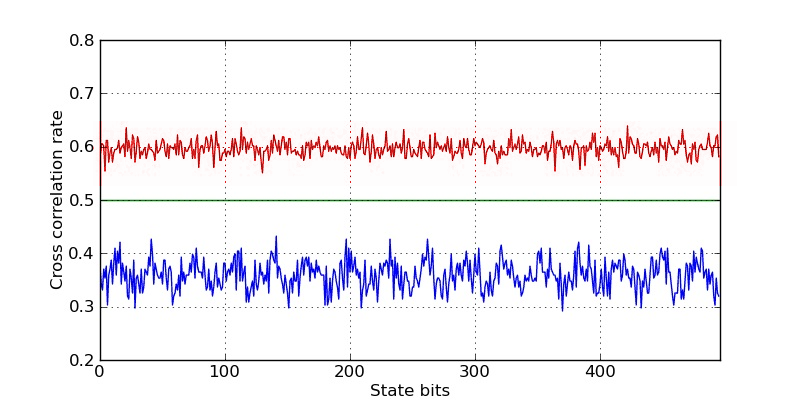
\includegraphics[scale=0.5]{correlation}
        \caption{Взаємна кореляція стану регістру до та після ініціалізації}
        \label{fig:corr}
    \end{figure}
\end{frame}

\begin{frame}{Поточний шифр ZUC}{Випадковість гами шифруючої}
    \begin{block}{}
        \begin{itemize}
            \item $55$ зразків гами по $65504$ біти з довгими бітовими серіями;
            \item виконано $163 / 189$ тестів;
            \item успішно пройдено $162$ тести.
        \end{itemize}
    \end{block}
    \begin{figure}[htbp]
        \centering
        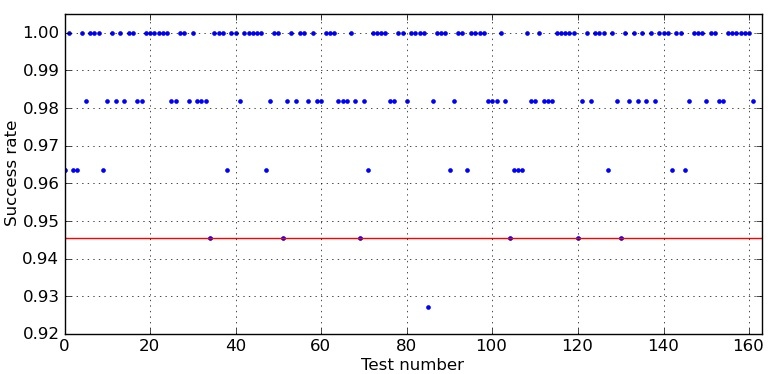
\includegraphics[scale=0.5]{stats}
        \caption{Результати тестування випадковості гами шифруючої}
        \label{fig:corr}
    \end{figure}
\end{frame}

\begin{frame}{Поточний шифр ZUC}{Результати аналізу}
    \small
    \begin{block}{Підсумки}
        \begin{itemize}
            \item виявлено недолік лінійного перетворення ZUC;
            \item структура шифру не дозволяє використати властивість для атаки;
            \item лінійне перетворення необхідно вдосконалити перед
                використанням в інших перспективних криптоалгоритмах;
            \item спостерігається відхилення взаємної кореляції станів регістру
                від випадкових значень на ключах з довгими бітовими серіями;
            \item гама шифруюча відповідає критеріям випадковості згідно NIST~STS.
        \end{itemize}
    \end{block}
    \begin{block}{Вдалі криптографічні рішення}
        \begin{itemize}
            \item комбінування XOR та додавання за модулем;
            \item перемішування станів регістрів кінцевого автомату;
            \item складання вихідних слів кінцевого автомату з бітами регістру
                зсуву.
        \end{itemize}
    \end{block}
\end{frame}


\section{Огляд вимог та аналіз властивостей перспективного шифра для компактної реалізації}
\begin{frame}{Мало-ресурсна криптографія}{Шифр PRESENT}
    \small
    \begin{minipage}[t]{0.65\textwidth}
        \begin{itemize}
            \item 64-бітний блок даних.
            \item Блоки заміни: S-блок $F_2^4 \rightarrow F_2^4$. \\
            \item Бітове перемішування: 
                \begin{equation}
                    \label{eqn:player}
                    \nonumber
                    P(i) = \left\{
                    \begin{array}{ll}
                        i \cdot 16 \mod 63, & i \in {0, \hdots, 62} \\
                        63,  & i = 63 \enspace.
                    \end{array} \right.
                \end{equation}
            \item 31 раунд + відбілювання ключа.
            \item Довжина майстер-ключа --- \\
                80 або 128 бітів.
            \item Розгортання ключів:
                \begin{enumerate}
                    \setlength{\itemsep}{1pt}
                        \setlength{\parskip}{0pt}
                        \setlength{\parsep}{0pt}
                    \item $ [k_{79} k_{78} \hdots k_1 k_0] = [k_{18} k_{17} \hdots k_{20} k_{19}] $;
                    \item $ [K_{79} k_{78} k_{77} k_{76}] = S[k_{79} k_{78} k_{77} k_{76}] $;
                    \item $ [k_{19} k_{18} k_{17} k_{16} k_{15}] = [k_{19} k_{18} k_{17} k_{16} k_{15} 
                        \oplus \mbox{round\_counter}] $.
                \end{enumerate}
        \end{itemize}
    \end{minipage}%
    \begin{minipage}[t]{0.35\linewidth}
        \begin{figure}[h]
            \centering
            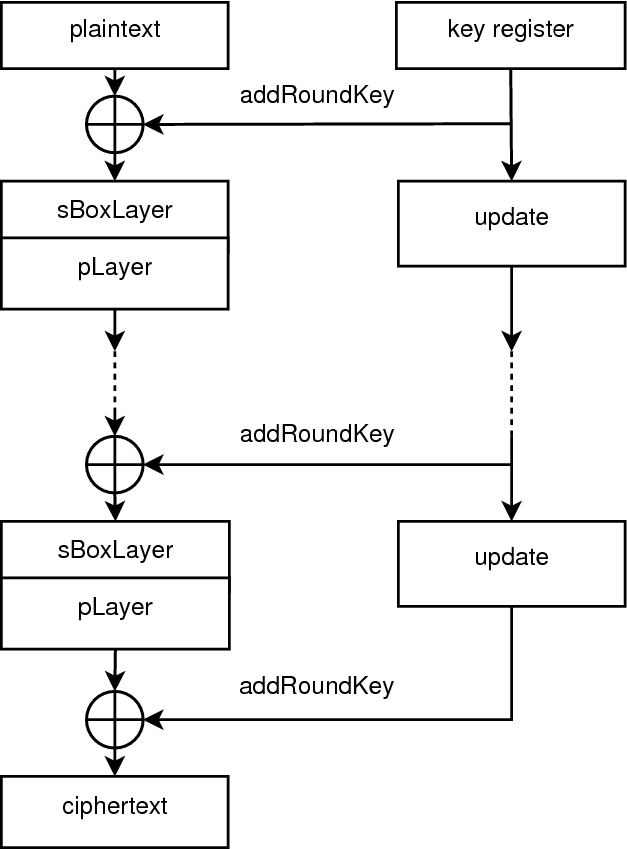
\includegraphics[scale=0.2]{present}
            \label{fig:present}
        \end{figure}
    \end{minipage}
\end{frame}

\begin{frame}{Мало-ресурсна криптографія}{Порівняння шифрів}
    \begin{block}{Обґрунтування}
        \begin{itemize}
            \item PRESENT розроблений для мало-ресурсної криптографії; \\
                став міжнародним стандартом: ISO/IEC~29192-2:2012;
            \item ГОСТ~28147 є стандартом шифрування у країнах СНД,
                доступний для криптоаналізу понад 20 років;
            \item AES є найбільш розповсюдженим блоковим симетричним шифром.
        \end{itemize}
    \end{block}
    \begin{table}[htbp]
        \centering
        \caption{Порівняння PRESENT, AES та ГОСТ~28147-89}
        \label{tbl:comparison}
        \begin{tabular}{|l|p{1cm}|p{1cm}|p{2cm}|p{1.2cm}|p{2cm}|}
            \hline
            Шифр  & ключ, біт & блок, біт & Швидкість, Kb/s & Площа, GE & Ефективність, $\frac{bps}{\text{GE}}$ \\
            \hline
            PRESENT & 80  & 64  & 11.7 & 1075 & 10.89 \\
            \hline
            ГОСТ    & 256 & 64  & 14   & 800  & 17.5  \\
            \hline
            AES     & 128 & 128 & 80   & 3100 & 25.81 \\
            \hline
        \end{tabular}
    \end{table}
\end{frame}

\section{Алгебраїчний криптоаналіз  ГОСТ~28147}
\begin{frame}{Алгебраїчний криптоаналіз}
    \begin{block}{Клод Шеннон}
        ``Злам стійкого шифру має потребувати такий же обсяг обчислень, що і
        вирішення системи рівнянь від багатьох невідомих''.
    \end{block}
    \begin{minipage}[t]{0.5\textwidth}
        \begin{block}{Основні принципи}
            \begin{enumerate}
                \item криптоалгоритм описується системою рівнянь другого
                    степеня від багатьох змінних;
                \item за наявності відкритих повідомлень та шифротекстів,
                    система рівнянь вирішується для знаходження бітів ключа.
            \end{enumerate}
        \end{block}
    \end{minipage}%
    \hspace*{1ex}
    \begin{minipage}[t]{0.5\textwidth}
        \begin{figure}[htbp]
            \centering
            % Graphic for TeX using PGF
% Title: /home/zoresvit/Documents/diploma/bachelor-thesis/images/gost.dia
% Creator: Dia v0.97.1
% CreationDate: Wed May  9 22:47:17 2012
% For: zoresvit
% \usepackage{tikz}
% The following commands are not supported in PSTricks at present
% We define them conditionally, so when they are implemented,
% this pgf file will use them.
\ifx\du\undefined
  \newlength{\du}
\fi
\setlength{\du}{15\unitlength}
\begin{tikzpicture}[scale=0.55,every node/.style={scale=0.6}]
\pgftransformxscale{1.000000}
\pgftransformyscale{-1.000000}
\definecolor{dialinecolor}{rgb}{0.000000, 0.000000, 0.000000}
\pgfsetstrokecolor{dialinecolor}
\definecolor{dialinecolor}{rgb}{1.000000, 1.000000, 1.000000}
\pgfsetfillcolor{dialinecolor}
\definecolor{dialinecolor}{rgb}{1.000000, 1.000000, 1.000000}
\pgfsetfillcolor{dialinecolor}
\fill (16.000000\du,2.000000\du)--(16.000000\du,4.000000\du)--(28.000000\du,4.000000\du)--(28.000000\du,2.000000\du)--cycle;
\pgfsetlinewidth{0.100000\du}
\pgfsetdash{}{0pt}
\pgfsetdash{}{0pt}
\pgfsetmiterjoin
\definecolor{dialinecolor}{rgb}{0.000000, 0.000000, 0.000000}
\pgfsetstrokecolor{dialinecolor}
\draw (16.000000\du,2.000000\du)--(16.000000\du,4.000000\du)--(28.000000\du,4.000000\du)--(28.000000\du,2.000000\du)--cycle;
% setfont left to latex
\definecolor{dialinecolor}{rgb}{0.000000, 0.000000, 0.000000}
\pgfsetstrokecolor{dialinecolor}
\node at (22.000000\du,3.000000\du){INPUT};
\definecolor{dialinecolor}{rgb}{1.000000, 1.000000, 1.000000}
\pgfsetfillcolor{dialinecolor}
\fill (16.000000\du,12.000000\du)--(16.000000\du,14.000000\du)--(28.000000\du,14.000000\du)--(28.000000\du,12.000000\du)--cycle;
\pgfsetlinewidth{0.100000\du}
\pgfsetdash{}{0pt}
\pgfsetdash{}{0pt}
\pgfsetmiterjoin
\definecolor{dialinecolor}{rgb}{0.000000, 0.000000, 0.000000}
\pgfsetstrokecolor{dialinecolor}
\draw (16.000000\du,12.000000\du)--(16.000000\du,14.000000\du)--(28.000000\du,14.000000\du)--(28.000000\du,12.000000\du)--cycle;
% setfont left to latex
\definecolor{dialinecolor}{rgb}{0.000000, 0.000000, 0.000000}
\pgfsetstrokecolor{dialinecolor}
\node at (22.000000\du,13.000000\du){OUTPUT};
\definecolor{dialinecolor}{rgb}{1.000000, 1.000000, 1.000000}
\pgfsetfillcolor{dialinecolor}
\fill (30.000000\du,2.000000\du)--(30.000000\du,4.000000\du)--(36.000000\du,4.000000\du)--(36.000000\du,2.000000\du)--cycle;
\pgfsetlinewidth{0.100000\du}
\pgfsetdash{}{0pt}
\pgfsetdash{}{0pt}
\pgfsetmiterjoin
\definecolor{dialinecolor}{rgb}{0.000000, 0.000000, 0.000000}
\pgfsetstrokecolor{dialinecolor}
\draw (30.000000\du,2.000000\du)--(30.000000\du,4.000000\du)--(36.000000\du,4.000000\du)--(36.000000\du,2.000000\du)--cycle;
% setfont left to latex
\definecolor{dialinecolor}{rgb}{0.000000, 0.000000, 0.000000}
\pgfsetstrokecolor{dialinecolor}
\node at (33.000000\du,3.000000\du){SUBKEY};
\pgfsetlinewidth{0.100000\du}
\pgfsetdash{}{0pt}
\pgfsetdash{}{0pt}
\pgfsetbuttcap
{
\definecolor{dialinecolor}{rgb}{0.000000, 0.000000, 0.000000}
\pgfsetfillcolor{dialinecolor}
% was here!!!
\definecolor{dialinecolor}{rgb}{0.000000, 0.000000, 0.000000}
\pgfsetstrokecolor{dialinecolor}
\draw (26.500000\du,4.500000\du)--(26.500000\du,8.000000\du);
}
\pgfsetlinewidth{0.100000\du}
\pgfsetdash{}{0pt}
\pgfsetdash{}{0pt}
\pgfsetmiterjoin
\pgfsetbuttcap
{
\definecolor{dialinecolor}{rgb}{0.000000, 0.000000, 0.000000}
\pgfsetfillcolor{dialinecolor}
% was here!!!
{\pgfsetcornersarced{\pgfpoint{0.000000\du}{0.000000\du}}\definecolor{dialinecolor}{rgb}{0.000000, 0.000000, 0.000000}
\pgfsetstrokecolor{dialinecolor}
\draw (33.000000\du,4.000000\du)--(33.000000\du,5.500000\du)--(26.754900\du,5.500000\du)--(26.754900\du,5.500000\du);
}}
\pgfsetlinewidth{0.100000\du}
\pgfsetdash{}{0pt}
\pgfsetdash{}{0pt}
\pgfsetmiterjoin
\definecolor{dialinecolor}{rgb}{1.000000, 1.000000, 1.000000}
\pgfsetfillcolor{dialinecolor}
\fill (24.800000\du,6.500000\du)--(24.800000\du,7.500000\du)--(25.800000\du,7.500000\du)--(25.800000\du,6.500000\du)--cycle;
\definecolor{dialinecolor}{rgb}{0.000000, 0.000000, 0.000000}
\pgfsetstrokecolor{dialinecolor}
\draw (24.800000\du,6.500000\du)--(24.800000\du,7.500000\du)--(25.800000\du,7.500000\du)--(25.800000\du,6.500000\du)--cycle;
\pgfsetlinewidth{0.100000\du}
\pgfsetdash{}{0pt}
\pgfsetdash{}{0pt}
\pgfsetbuttcap
{
\definecolor{dialinecolor}{rgb}{0.000000, 0.000000, 0.000000}
\pgfsetfillcolor{dialinecolor}
% was here!!!
\definecolor{dialinecolor}{rgb}{0.000000, 0.000000, 0.000000}
\pgfsetstrokecolor{dialinecolor}
\draw (25.300000\du,6.500000\du)--(25.300000\du,7.500000\du);
}
\pgfsetlinewidth{0.100000\du}
\pgfsetdash{}{0pt}
\pgfsetdash{}{0pt}
\pgfsetbuttcap
{
\definecolor{dialinecolor}{rgb}{0.000000, 0.000000, 0.000000}
\pgfsetfillcolor{dialinecolor}
% was here!!!
\definecolor{dialinecolor}{rgb}{0.000000, 0.000000, 0.000000}
\pgfsetstrokecolor{dialinecolor}
\draw (24.800000\du,7.000000\du)--(25.800000\du,7.000000\du);
}
% setfont left to latex
\definecolor{dialinecolor}{rgb}{0.000000, 0.000000, 0.000000}
\pgfsetstrokecolor{dialinecolor}
\node[anchor=west] at (27.200000\du,1.500000\du){0};
% setfont left to latex
\definecolor{dialinecolor}{rgb}{0.000000, 0.000000, 0.000000}
\pgfsetstrokecolor{dialinecolor}
\node[anchor=west] at (20.500000\du,1.500000\du){32 31};
% setfont left to latex
\definecolor{dialinecolor}{rgb}{0.000000, 0.000000, 0.000000}
\pgfsetstrokecolor{dialinecolor}
\node[anchor=west] at (15.500000\du,1.500000\du){63};
% setfont left to latex
\definecolor{dialinecolor}{rgb}{0.000000, 0.000000, 0.000000}
\pgfsetstrokecolor{dialinecolor}
\node[anchor=west] at (35.200000\du,1.500000\du){0};
% setfont left to latex
\definecolor{dialinecolor}{rgb}{0.000000, 0.000000, 0.000000}
\pgfsetstrokecolor{dialinecolor}
\node[anchor=west] at (29.500000\du,1.500000\du){31};
\pgfsetlinewidth{0.100000\du}
\pgfsetdash{}{0pt}
\pgfsetdash{}{0pt}
\pgfsetbuttcap
{
\definecolor{dialinecolor}{rgb}{0.000000, 0.000000, 0.000000}
\pgfsetfillcolor{dialinecolor}
% was here!!!
\definecolor{dialinecolor}{rgb}{0.000000, 0.000000, 0.000000}
\pgfsetstrokecolor{dialinecolor}
\pgfpathmoveto{\pgfpoint{26.800000\du}{5.546870\du}}
\pgfpatharc{360}{181}{0.300000\du and 0.300000\du}
\pgfusepath{stroke}
}
% setfont left to latex
\definecolor{dialinecolor}{rgb}{0.000000, 0.000000, 0.000000}
\pgfsetstrokecolor{dialinecolor}
\node[anchor=west] at (33.500000\du,5.000000\du){$K_i$};
\pgfsetlinewidth{0.100000\du}
\pgfsetdash{}{0pt}
\pgfsetdash{}{0pt}
\pgfsetbuttcap
{
\definecolor{dialinecolor}{rgb}{0.000000, 0.000000, 0.000000}
\pgfsetfillcolor{dialinecolor}
% was here!!!
\definecolor{dialinecolor}{rgb}{0.000000, 0.000000, 0.000000}
\pgfsetstrokecolor{dialinecolor}
\draw (26.500000\du,8.000000\du)--(17.500000\du,9.500000\du);
}
\pgfsetlinewidth{0.100000\du}
\pgfsetdash{}{0pt}
\pgfsetdash{}{0pt}
\pgfsetmiterjoin
\pgfsetbuttcap
{
\definecolor{dialinecolor}{rgb}{0.000000, 0.000000, 0.000000}
\pgfsetfillcolor{dialinecolor}
% was here!!!
\definecolor{dialinecolor}{rgb}{0.000000, 0.000000, 0.000000}
\pgfsetstrokecolor{dialinecolor}
\pgfpathmoveto{\pgfpoint{26.500000\du}{4.500000\du}}
\pgfpathcurveto{\pgfpoint{26.500000\du}{3.900000\du}}{\pgfpoint{22.000000\du}{4.600000\du}}{\pgfpoint{22.000000\du}{4.000000\du}}
\pgfusepath{stroke}
}
\pgfsetlinewidth{0.100000\du}
\pgfsetdash{}{0pt}
\pgfsetdash{}{0pt}
\pgfsetmiterjoin
\pgfsetbuttcap
{
\definecolor{dialinecolor}{rgb}{0.000000, 0.000000, 0.000000}
\pgfsetfillcolor{dialinecolor}
% was here!!!
\definecolor{dialinecolor}{rgb}{0.000000, 0.000000, 0.000000}
\pgfsetstrokecolor{dialinecolor}
\pgfpathmoveto{\pgfpoint{26.500000\du}{4.500000\du}}
\pgfpathcurveto{\pgfpoint{26.500000\du}{4.100000\du}}{\pgfpoint{28.000000\du}{4.600000\du}}{\pgfpoint{28.000000\du}{4.000000\du}}
\pgfusepath{stroke}
}
\pgfsetlinewidth{0.100000\du}
\pgfsetdash{}{0pt}
\pgfsetdash{}{0pt}
\pgfsetmiterjoin
\pgfsetbuttcap
{
\definecolor{dialinecolor}{rgb}{0.000000, 0.000000, 0.000000}
\pgfsetfillcolor{dialinecolor}
% was here!!!
\definecolor{dialinecolor}{rgb}{0.000000, 0.000000, 0.000000}
\pgfsetstrokecolor{dialinecolor}
\pgfpathmoveto{\pgfpoint{17.500000\du}{11.500000\du}}
\pgfpathcurveto{\pgfpoint{17.500000\du}{11.880000\du}}{\pgfpoint{16.000000\du}{11.500000\du}}{\pgfpoint{16.000000\du}{12.000000\du}}
\pgfusepath{stroke}
}
\pgfsetlinewidth{0.100000\du}
\pgfsetdash{}{0pt}
\pgfsetdash{}{0pt}
\pgfsetmiterjoin
\pgfsetbuttcap
{
\definecolor{dialinecolor}{rgb}{0.000000, 0.000000, 0.000000}
\pgfsetfillcolor{dialinecolor}
% was here!!!
\definecolor{dialinecolor}{rgb}{0.000000, 0.000000, 0.000000}
\pgfsetstrokecolor{dialinecolor}
\pgfpathmoveto{\pgfpoint{17.500000\du}{11.500000\du}}
\pgfpathcurveto{\pgfpoint{17.500000\du}{12.100000\du}}{\pgfpoint{22.000000\du}{11.300000\du}}{\pgfpoint{22.000000\du}{12.000000\du}}
\pgfusepath{stroke}
}
\pgfsetlinewidth{0.100000\du}
\pgfsetdash{}{0pt}
\pgfsetdash{}{0pt}
\pgfsetbuttcap
{
\definecolor{dialinecolor}{rgb}{0.000000, 0.000000, 0.000000}
\pgfsetfillcolor{dialinecolor}
% was here!!!
\pgfsetarrowsend{stealth}
\definecolor{dialinecolor}{rgb}{0.000000, 0.000000, 0.000000}
\pgfsetstrokecolor{dialinecolor}
\draw (17.500000\du,9.500000\du)--(17.500000\du,11.500000\du);
}
\definecolor{dialinecolor}{rgb}{1.000000, 1.000000, 1.000000}
\pgfsetfillcolor{dialinecolor}
\fill (21.700000\du,6.175000\du)--(21.700000\du,7.804167\du)--(23.982500\du,7.804167\du)--(23.982500\du,6.175000\du)--cycle;
\pgfsetlinewidth{0.100000\du}
\pgfsetdash{}{0pt}
\pgfsetdash{}{0pt}
\pgfsetmiterjoin
\definecolor{dialinecolor}{rgb}{0.000000, 0.000000, 0.000000}
\pgfsetstrokecolor{dialinecolor}
\draw (21.700000\du,6.175000\du)--(21.700000\du,7.804167\du)--(23.982500\du,7.804167\du)--(23.982500\du,6.175000\du)--cycle;
% setfont left to latex
\definecolor{dialinecolor}{rgb}{0.000000, 0.000000, 0.000000}
\pgfsetstrokecolor{dialinecolor}
\node at (22.841250\du,7.120000\du){S-box};
\pgfsetlinewidth{0.100000\du}
\pgfsetdash{}{0pt}
\pgfsetdash{}{0pt}
\pgfsetmiterjoin
\pgfsetbuttcap
{
\definecolor{dialinecolor}{rgb}{0.000000, 0.000000, 0.000000}
\pgfsetfillcolor{dialinecolor}
% was here!!!
\pgfsetarrowsend{stealth}
{\pgfsetcornersarced{\pgfpoint{0.000000\du}{0.000000\du}}\definecolor{dialinecolor}{rgb}{0.000000, 0.000000, 0.000000}
\pgfsetstrokecolor{dialinecolor}
\draw (26.247900\du,5.500000\du)--(26.247900\du,5.500000\du)--(25.300000\du,5.500000\du)--(25.300000\du,6.455078\du);
}}
\pgfsetlinewidth{0.100000\du}
\pgfsetdash{}{0pt}
\pgfsetdash{}{0pt}
\pgfsetbuttcap
{
\definecolor{dialinecolor}{rgb}{0.000000, 0.000000, 0.000000}
\pgfsetfillcolor{dialinecolor}
% was here!!!
\pgfsetarrowsend{stealth}
\definecolor{dialinecolor}{rgb}{0.000000, 0.000000, 0.000000}
\pgfsetstrokecolor{dialinecolor}
\draw (24.800000\du,7.000000\du)--(23.982500\du,6.989583\du);
}
\pgfsetlinewidth{0.100000\du}
\pgfsetdash{}{0pt}
\pgfsetdash{}{0pt}
\pgfsetmiterjoin
\pgfsetbuttcap
{
\definecolor{dialinecolor}{rgb}{0.000000, 0.000000, 0.000000}
\pgfsetfillcolor{dialinecolor}
% was here!!!
\definecolor{dialinecolor}{rgb}{0.000000, 0.000000, 0.000000}
\pgfsetstrokecolor{dialinecolor}
\pgfpathmoveto{\pgfpoint{17.500000\du}{4.500000\du}}
\pgfpathcurveto{\pgfpoint{17.500000\du}{4.100000\du}}{\pgfpoint{16.000000\du}{4.600000\du}}{\pgfpoint{16.000000\du}{4.000000\du}}
\pgfusepath{stroke}
}
\pgfsetlinewidth{0.100000\du}
\pgfsetdash{}{0pt}
\pgfsetdash{}{0pt}
\pgfsetmiterjoin
\pgfsetbuttcap
{
\definecolor{dialinecolor}{rgb}{0.000000, 0.000000, 0.000000}
\pgfsetfillcolor{dialinecolor}
% was here!!!
\definecolor{dialinecolor}{rgb}{0.000000, 0.000000, 0.000000}
\pgfsetstrokecolor{dialinecolor}
\pgfpathmoveto{\pgfpoint{17.500000\du}{4.500000\du}}
\pgfpathcurveto{\pgfpoint{17.500000\du}{4.000000\du}}{\pgfpoint{22.000000\du}{4.600000\du}}{\pgfpoint{22.000000\du}{4.000000\du}}
\pgfusepath{stroke}
}
\pgfsetlinewidth{0.100000\du}
\pgfsetdash{}{0pt}
\pgfsetdash{}{0pt}
\pgfsetmiterjoin
\definecolor{dialinecolor}{rgb}{1.000000, 1.000000, 1.000000}
\pgfsetfillcolor{dialinecolor}
\fill (18.800000\du,6.487500\du)--(18.800000\du,7.487500\du)--(20.800000\du,7.487500\du)--(20.800000\du,6.487500\du)--cycle;
\definecolor{dialinecolor}{rgb}{0.000000, 0.000000, 0.000000}
\pgfsetstrokecolor{dialinecolor}
\draw (18.800000\du,6.487500\du)--(18.800000\du,7.487500\du)--(20.800000\du,7.487500\du)--(20.800000\du,6.487500\du)--cycle;
% setfont left to latex
\definecolor{dialinecolor}{rgb}{0.000000, 0.000000, 0.000000}
\pgfsetstrokecolor{dialinecolor}
\node[anchor=west] at (18.600000\du,7.000000\du){$<<<$};
\pgfsetlinewidth{0.100000\du}
\pgfsetdash{}{0pt}
\pgfsetdash{}{0pt}
\pgfsetbuttcap
{
\definecolor{dialinecolor}{rgb}{0.000000, 0.000000, 0.000000}
\pgfsetfillcolor{dialinecolor}
% was here!!!
\pgfsetarrowsend{stealth}
\definecolor{dialinecolor}{rgb}{0.000000, 0.000000, 0.000000}
\pgfsetstrokecolor{dialinecolor}
\draw (21.700000\du,6.989583\du)--(20.800000\du,6.987500\du);
}
\pgfsetlinewidth{0.100000\du}
\pgfsetdash{}{0pt}
\pgfsetdash{}{0pt}
\pgfsetbuttcap
\pgfsetmiterjoin
\pgfsetlinewidth{0.100000\du}
\pgfsetbuttcap
\pgfsetmiterjoin
\pgfsetdash{}{0pt}
\definecolor{dialinecolor}{rgb}{1.000000, 1.000000, 1.000000}
\pgfsetfillcolor{dialinecolor}
\pgfpathellipse{\pgfpoint{17.500000\du}{7.000000\du}}{\pgfpoint{0.500000\du}{0\du}}{\pgfpoint{0\du}{0.500000\du}}
\pgfusepath{fill}
\definecolor{dialinecolor}{rgb}{0.000000, 0.000000, 0.000000}
\pgfsetstrokecolor{dialinecolor}
\pgfpathellipse{\pgfpoint{17.500000\du}{7.000000\du}}{\pgfpoint{0.500000\du}{0\du}}{\pgfpoint{0\du}{0.500000\du}}
\pgfusepath{stroke}
\pgfsetbuttcap
\pgfsetmiterjoin
\pgfsetdash{}{0pt}
\definecolor{dialinecolor}{rgb}{0.000000, 0.000000, 0.000000}
\pgfsetstrokecolor{dialinecolor}
\draw (17.500000\du,6.500000\du)--(17.500000\du,7.500000\du);
\pgfsetbuttcap
\pgfsetmiterjoin
\pgfsetdash{}{0pt}
\definecolor{dialinecolor}{rgb}{0.000000, 0.000000, 0.000000}
\pgfsetstrokecolor{dialinecolor}
\draw (17.000000\du,7.000000\du)--(18.000000\du,7.000000\du);
\pgfsetlinewidth{0.100000\du}
\pgfsetdash{}{0pt}
\pgfsetdash{}{0pt}
\pgfsetbuttcap
{
\definecolor{dialinecolor}{rgb}{0.000000, 0.000000, 0.000000}
\pgfsetfillcolor{dialinecolor}
% was here!!!
\pgfsetarrowsend{stealth}
\definecolor{dialinecolor}{rgb}{0.000000, 0.000000, 0.000000}
\pgfsetstrokecolor{dialinecolor}
\draw (18.800000\du,6.987500\du)--(18.000000\du,7.000000\du);
}
\pgfsetlinewidth{0.100000\du}
\pgfsetdash{}{0pt}
\pgfsetdash{}{0pt}
\pgfsetbuttcap
{
\definecolor{dialinecolor}{rgb}{0.000000, 0.000000, 0.000000}
\pgfsetfillcolor{dialinecolor}
% was here!!!
\definecolor{dialinecolor}{rgb}{0.000000, 0.000000, 0.000000}
\pgfsetstrokecolor{dialinecolor}
\draw (17.500000\du,4.500000\du)--(17.500000\du,6.500000\du);
}
\pgfsetlinewidth{0.100000\du}
\pgfsetdash{}{0pt}
\pgfsetdash{}{0pt}
\pgfsetbuttcap
{
\definecolor{dialinecolor}{rgb}{0.000000, 0.000000, 0.000000}
\pgfsetfillcolor{dialinecolor}
% was here!!!
\definecolor{dialinecolor}{rgb}{0.000000, 0.000000, 0.000000}
\pgfsetstrokecolor{dialinecolor}
\draw (17.500000\du,7.500000\du)--(17.500000\du,8.000000\du);
}
\pgfsetlinewidth{0.100000\du}
\pgfsetdash{}{0pt}
\pgfsetdash{}{0pt}
\pgfsetbuttcap
{
\definecolor{dialinecolor}{rgb}{0.000000, 0.000000, 0.000000}
\pgfsetfillcolor{dialinecolor}
% was here!!!
\definecolor{dialinecolor}{rgb}{0.000000, 0.000000, 0.000000}
\pgfsetstrokecolor{dialinecolor}
\draw (17.500000\du,8.000000\du)--(26.500000\du,9.500000\du);
}
\pgfsetlinewidth{0.100000\du}
\pgfsetdash{}{0pt}
\pgfsetdash{}{0pt}
\pgfsetmiterjoin
\pgfsetbuttcap
{
\definecolor{dialinecolor}{rgb}{0.000000, 0.000000, 0.000000}
\pgfsetfillcolor{dialinecolor}
% was here!!!
\definecolor{dialinecolor}{rgb}{0.000000, 0.000000, 0.000000}
\pgfsetstrokecolor{dialinecolor}
\pgfpathmoveto{\pgfpoint{26.500000\du}{11.500000\du}}
\pgfpathcurveto{\pgfpoint{26.500000\du}{12.000000\du}}{\pgfpoint{22.000000\du}{11.300000\du}}{\pgfpoint{22.000000\du}{12.000000\du}}
\pgfusepath{stroke}
}
\pgfsetlinewidth{0.100000\du}
\pgfsetdash{}{0pt}
\pgfsetdash{}{0pt}
\pgfsetmiterjoin
\pgfsetbuttcap
{
\definecolor{dialinecolor}{rgb}{0.000000, 0.000000, 0.000000}
\pgfsetfillcolor{dialinecolor}
% was here!!!
\definecolor{dialinecolor}{rgb}{0.000000, 0.000000, 0.000000}
\pgfsetstrokecolor{dialinecolor}
\pgfpathmoveto{\pgfpoint{26.500000\du}{11.500000\du}}
\pgfpathcurveto{\pgfpoint{26.500000\du}{11.900000\du}}{\pgfpoint{28.000000\du}{11.400000\du}}{\pgfpoint{28.000000\du}{12.000000\du}}
\pgfusepath{stroke}
}
\pgfsetlinewidth{0.100000\du}
\pgfsetdash{}{0pt}
\pgfsetdash{}{0pt}
\pgfsetbuttcap
{
\definecolor{dialinecolor}{rgb}{0.000000, 0.000000, 0.000000}
\pgfsetfillcolor{dialinecolor}
% was here!!!
\pgfsetarrowsend{stealth}
\definecolor{dialinecolor}{rgb}{0.000000, 0.000000, 0.000000}
\pgfsetstrokecolor{dialinecolor}
\draw (26.500000\du,9.500000\du)--(26.500000\du,11.500000\du);
}
\pgfsetlinewidth{0.100000\du}
\pgfsetdash{}{0pt}
\pgfsetdash{}{0pt}
\pgfsetbuttcap
{
\definecolor{dialinecolor}{rgb}{0.000000, 0.000000, 0.000000}
\pgfsetfillcolor{dialinecolor}
% was here!!!
\pgfsetarrowsend{stealth}
\definecolor{dialinecolor}{rgb}{0.000000, 0.000000, 0.000000}
\pgfsetstrokecolor{dialinecolor}
\draw (26.500000\du,7.000000\du)--(25.800000\du,7.000000\du);
\node at (24.500000\du,5.500000\du){$Y_i$};
\node at (24.000000\du,3.000000\du){$X_i$};
\node at (21.000000\du,5.700000\du){$Z_i$};
\node at (25.000000\du,13.100000\du){$X_{i+1}$};
}
\end{tikzpicture}

            \caption{Циклова функція ГОСТ~28147-89}
        \end{figure}
    \end{minipage}%
\end{frame}

\begin{frame}[fragile, shrink]{Алгебраїчний криптоаналіз}{Вирішення алгебраїчних рівнянь}
    \small
    \begin{block}{Система рівнянь ГОСТ~28147-89}
        \begin{itemize}
            \item реалізовано з використанням системи символьної алгебри SAGE;
            \item один раунд шифру містить $325$ рівнянь другого степеня;
            \item повний шифр описується $10432$ поліномами від $4416$ змінних;
            \item можливо вирішити алгебраїчну систему для $5$ раундів ГОСТ~28147-89.
        \end{itemize}
    \end{block}

    \begin{block}{Використання CryptoMiniSat}
    \begin{enumerate}
        \item формується система рівнянь шифра в АНФ за допомогою SAGE;
        \item система рівнянь конвертується з АНФ формату до КНФ;
        \item \verb+CryptoMiniSat+ знаходить набір змінних, що задовольняє систему рівнянь. 
    \end{enumerate} 
    \end{block}
    \begin{example}
\begin{lstlisting}
sage: gost = Gost(rounds=5)
sage: f = gost.polynomial_system()
sage: solver = ANFSatSolver(f.ring())
sage: s, t = solver(f)
\end{lstlisting}
    \end{example}
\end{frame}

\begin{frame}{Висновки}
    \footnotesize
    \begin{block}{Аналіз шифра ZUC}
        \begin{itemize}
            \item досліджено криптографічні властивості шифра та розглянуто
                недолік лінійного перетворення;
            \item дослідження шифра не виявило практичних вразливостей
                алгоритму.
        \end{itemize}
    \end{block}

    \begin{block}{Мало-ресурсна криптографія}
        \begin{itemize}
            \item хоча ГОСТ~28147 використовується більше 20 років, він задовольняє
                усім вимогам шифра, націленого на компактну реалізацію (іноді краще за PRESENT);
            \item можлива реалізація шифра ГОСТ з використанням 800 вентильних еквівалентів.
        \end{itemize}
    \end{block}

    \begin{block}{Алгебраїчний криптоаналіз}
        \begin{itemize}
            \item алгоритм ГОСТ вдало описується системою рівнянь другого степеня;
            \item на даний момент можливо вирішити алгебраїчну систему, що
                описує 5 раундів шифрування ГОСТ~28147;
            \item подальша оптимізація може дозволити успішно вирішити алгебраїчну систему
                для більшої кількості раундів.
        \end{itemize} 
    \end{block}
\end{frame}

\begin{frame}[allowframebreaks]{Список публікацій}
    \scriptsize
    \begingroup
    \renewcommand{\chapter}[2]{}%
    \begin{thebibliography}{1}
            \providecommand*{\BibEmph}[1]{#1}
            \providecommand*{\cyrdash}{\hbox to.8em{--\hss--}}
            \providecommand*{\BibDash}{\ifdim\lastskip>0pt\unskip\nobreak\hskip.2em\fi\cyrdash\hskip.2em\ignorespaces}

            \bibitem{Kiyanchuk:DESSERT:2012}
            \BibEmph{Oliynykov~R.~V., Kiyanchuk~R.~I.} 
            \newblock {Perspective Symmetric Block Cipher optimized for Hardware Implementation}~// 
            \newblock {6-th International Conference ``Dependable Systems, Services \& Technologies (DESSERT'12)''}. \BibDash 2012.

            \bibitem{Kiyanchuk:visnyk:2012}
            \BibEmph{Kiyanchuk~R.~I., Oliynykov~R.~V.} \newblock {Linear transformation properties of
            ZUC cipher}~// \newblock \BibEmph{Visnyk}. \BibDash 2012. \BibDash{Mathematical modeling. Information technologies. Computer-aided
            control systems.}

            \bibitem{karazina:zuc}
            \BibEmph{{Kiyanchuk, R. I. and Oliynykov R. V.}} \newblock {Linear transformation
            properties of ZUC cipher}~// \newblock {Computer modeling in high-end technologies}~/
            Kharkiv national university of radio electronics. \BibDash {Kharkiv}, 2012. \BibDash P.~199 -- 202.

            \bibitem{Kiyanchuk:2012:Banking}
            \BibEmph{Кіянчук~Р.~І.} \newblock {Диференційний аналіз S-функцій}~// 
            \newblock {Наукові дослідження молоді вирішенню проблем європейської інтеграції}~/
            Харківський університет банківської справи. \BibDash Харків, 2012.
            \BibDash Електронне видання на CD-ROM.

            \bibitem{Kiyanchuk:2012:MMF}
            \BibEmph{Кіянчук~Р.~І.} \newblock {Диференційний аналіз S-функцій}~// 
            \newblock {Радіоелектроніка та молодь у XXI столітті}~/ Харківський
            національний університет радіоелектроніки. \BibDash Харків, 2012. \BibDash {с.}~130 -- 131.

            \bibitem{Kiyanchuk:2011:MMF}
            \BibEmph{Кіянчук~Р.~І.} \newblock {Порівняльний аналіз
            IDEA-подібних блочних симетричних шифрів}~// \newblock {
            Міжнародна конференція ``Комп'ютерна інженерія''}~/ 
            Харківський національний університет радіоелектроніки. \BibDash
            Харків, 2011. \BibDash {с.}~225 -- 227.

            \bibitem{Kiyanchuk:IREF:2011:present}
            \BibEmph{Олійников~Р.~В., Кіянчук~Р.~І.} 
            \newblock{Перспективний блочний симетричний шифр оптимізований для
            апаратної реалізації}~// 
            \newblock{Міжнародна конференція ``Телекомунікаційні системи та
            технології''}~/ 
            Харківський національний університет радіоелектроніки.
            \BibDash Т.~II. \BibDash {Харків, Україна}, 2011. \BibDash 
            с.~321 -- 330.


            \bibitem{Kiyanchuk:2011:Customs}
                \BibEmph{Олейников, Р.~В. and Киянчук, Р.~И.} 
                \newblock{Использование Т-функций в симметричных криптографических преобразованиях}~// 
                \newblock{Материалы международной научно-практической конференции <<Перспективы
	развития информационных и транспортно-таможенных технологий в таможенном
	деле, внешнеэкономической деятельности и управлении организациями>>}~/ 
    {Харьковский национальный университет радиоэлектроники}. \BibDash Днепропетровск, 2011. \BibDash 
            {c.}~213 -- 215.

            \bibitem{Kiyanchuk:2009:rijndael}
            \BibEmph{Долгов, В.~И. and Лисицкая, И.~В. and Киянчук, Р.~И.} 
            \newblock {RIJNDAEL -- это новое или хорошо забытое старое?}~// 
            \newblock{Компьютерные Науки и Технологии}~/ \BibDash
            2009. \BibDash с.~32 -- 35.
    \end{thebibliography}
\endgroup
\end{frame} 
\end{document}

